%%%%%%%%%%%%%%%%%%%%%%%%%%% asme2ej.tex %%%%%%%%%%%%%%%%%%%%%%%%%%%%%%%
% Template for producing ASME-format journal articles using LaTeX    %
% Written by   Harry H. Cheng, Professor and Director                %
%              Integration Engineering Laboratory                    %
%              Department of Mechanical and Aeronautical Engineering %
%              University of California                              %
%              Davis, CA 95616                                       %
%              Tel: (530) 752-5020 (office)                          %
%                   (530) 752-1028 (lab)                             %
%              Fax: (530) 752-4158                                   %
%              Email: hhcheng@ucdavis.edu                            %
%              WWW:   http://iel.ucdavis.edu/people/cheng.html       %
%              May 7, 1994                                           %
% Modified: February 16, 2001 by Harry H. Cheng                      %
% Modified: January  01, 2003 by Geoffrey R. Shiflett                %
% Use at your own risk, send complaints to /dev/null                 %
%%%%%%%%%%%%%%%%%%%%%%%%%%%%%%%%%%%%%%%%%%%%%%%%%%%%%%%%%%%%%%%%%%%%%%

%%% use twocolumn and 10pt options with the asme2ej format

\documentclass[twocolumn,10pt]{asme2ej}

\usepackage[none]{hyphenat}
\usepackage{epsfig} %% for loading postscript figures
\usepackage{amsmath}
\usepackage{amssymb}
\usepackage{breqn}

% color code for Octave/Matlab (thanks to SOUAD !)
\usepackage{listings} 
\usepackage{color} %red, green, blue, yellow, cyan, magenta, black, white
\definecolor{mygreen}{RGB}{28,172,0} % color values Red, Green, Blue
\definecolor{mylilas}{RGB}{170,55,241}


\lstset{language=Matlab,%
   %basicstyle=\color{red},
   breaklines=true,%
   morekeywords={Matlab2tikz},
   keywordstyle=\color{blue},%
   morekeywords=[2]{1}, keywordstyle=[2]{\color{black}},
   identifierstyle=\color{black},%
   stringstyle=\color{mylilas},
   commentstyle=\color{mygreen},%
   showstringspaces=false,%without this there will be a symbol in the places where there is a space
   numbers=left,%
   frame=trBL,
   numberstyle={\tiny \color{black}},% size of the numbers
   numbersep=9pt, % this defines how far the numbers are from the text
   emph=[1]{for,end,break},emphstyle=[1]\color{red}, %some words to emphasise
   %emph=[2]{word1,word2}, emphstyle=[2]{style},   
   }

\makeatletter
\lst@CCPutMacro
    \lst@ProcessOther {"2D}{\lst@ttfamily{-{}}{-}}
    \@empty\z@\@empty
\makeatother

\graphicspath{{./}{../../STABLE_CASES/CYLINDER/FIGURES/}{../../DEVELOPMENT_CASES/CompressibleCylinder/Sponge/FIGURES/}}

% previous way
%\usepackage{listings}
\usepackage[colorlinks, linkcolor=blue, citecolor=blue,filecolor=black,urlcolor=blue]{hyperref}



\newcommand{\be}[1]{ \begin{equation} \label{#1}}
\newcommand{\ee}{\end{equation}}


\newcommand{\bes}[1]{ \begin{equation} \label{#1}\begin{array}{rl}}
\newcommand{\ees}{\end{array}\end{equation}}



%% The class has several options
%  onecolumn/twocolumn - format for one or two columns per page
%  10pt/11pt/12pt - use 10, 11, or 12 point font
%  oneside/twoside - format for oneside/twosided printing
%  final/draft - format for final/draft copy
%  cleanfoot - take out copyright info in footer leave page number
%  cleanhead - take out the conference banner on the title page
%  titlepage/notitlepage - put in titlepage or leave out titlepage
%  
%% The default is oneside, onecolumn, 10pt, final


%\title{Popularizing linear and nonlinear global approaches to hydrodynamic instabilities: 
%A review and a simple implementation for the wake of a cylinder}

\title{A practical review on linear and nonlinear global approaches to flow instabilities}

%%% first author
\author{D. Fabre$^{(a)}$,  V. Citro$^{(b,a)}$,  D. Ferreira Sabino$^{(a)}$, P. Bonnefis$^{(a)}$,  J. Sierra $^{(a)}$, F. Giannetti$^{(b)}$ \& M. Pigou$^{(a)}$ 
    \affiliation{
	$^{(a)}$ Institut de M\'ecanique des fluides de Toulouse (IMFT), University of Toulouse \\
	$^{(b)}$ Dipartimento di Ingegneria (DIIN), Universit\'a} di Salerno. 
}

%%% second author
%%% remove the following entry for single author papers
%%% add more entries for additional authors
%\author{V. Citro$^{(b)}$ \& F. Giannetti$^{(b)}$ \\
 %   \affiliation{ University of Salerno
  %  }
%}

\usepackage{cprotect}

\begin{document}
\lstset{numbers=left, numberstyle=\small, numbersep=8pt, frame = single, language=Matlab, framexleftmargin=15pt}

\maketitle    

%%%%%%%%%%%%%%%%%%%%%%%%%%%%%%%%%%%%%%%%%%%%%%%%%%%%%%%%%%%%%%%%%%%%%%
\begin{abstract}
{\it 
This paper aims at reviewing linear and nonlinear approaches to study the stability of fluid flows. 
We provide a concise but self-contained exposition of the main concepts and specific numerical methods 
designed for global stability studies, including the classical linear stability analysis, the adjoint-based sensitivity and  
the most recent nonlinear developments. 
Regarding numerical implementation, a number of ideas making resolution particularly efficient are discussed, 
including mesh adaptation, simple shift-invert strategy instead of the classical Arnoldi algorithm, 
and a simplification of the recent nonlinear self-consistent approach proposed by Manti\v{c}-Lugo et al. (2014). 
An open-source software implementing all the concepts discussed in the present paper is provided. 
The software is demonstrated for the reference case of the two-dimensional flow around a circular cylinder, in both incompressible and compressible cases, but is easily customisable to a variety of other flow configurations or flow equations.
%An abstract for an ASME paper should be less than 150 words and is normally in italics.
}
\end{abstract}

%%%%%%%%%%%%%%%%%%%%%%%%%%%%%%%%%%%%%%%%%%%%%%%%%%%%%%%%%%%%%%%%%%%%%%


\section{Introduction}

The concept of stability bears on the response of a system to small perturbations of its state. If the generic disturbance grows in time, the system is unstable. The concept of stability can be simply formulated for a system of Ordinary Differential Equations (ODE). 
Such systems can be at equilibrium, where the state does not depend on time, or can present a periodic state, with all components returning to the same values, after every period. 

The stability of fluid flows usually depends on the value of a given parameter.
A bifurcation occurs when a critical value is reached and the original solution becomes linearly unstable, the system then starts evolving towards a new state, either steady or unsteady. 
In the second part of the 19th century, specific analytical and numerical methods have emerged to study these bifurcations and have continuously evolved up to the present days. 
A crucial point, that drove the development in this field, is the availability of significantly increasing and improving computing resources. 
Initially, the linear stability theory focused on fluid flows that are homogeneous in two spatial directions, \textit{e.g.} plane Poiseuille flow \cite{Dreid2004}. In this case, thanks to a Fourier decomposition in the two homogeneous directions, it is possible to reduce the stability problem to a one-dimensional problem, an approach usually referred to as {\em local stability approach}.
On the other hand,  when there are at least two spatial variables, the class of methods suited to solve such problems are generally called {\em global stability approaches}.
A classical example of such behaviour in fluid dynamics is the instability occurring in the wake of a circular cylinder. At low Reynolds number (precisely for $Re < 46.7$) the flow is steady and symmetric, but for larger values of Re a global instability arises in the flow field leading to the well-known von K\'arm\'an vortex alley. 
This flow configuration has served as a benchmark in the development of this class of methods.  
If one is only interested in predicting whether a flow is stable, it is sufficient to conduct a {\em linear stability analysis} which is the fundamental brick of global stability approaches. 
Beyond this simple question, in the past two decades, a number of extensions have been developed and popularized.
{\em Adjoint methods} are an important extension \cite{GiannettiLuchini},\cite{Marquet}; they can give insight into the sensitivity of the flow to intrinsic or extrinsic contributions. 
{\em Nonlinear stability approaches} \cite{SippLebedev} \cite{MLugo2014} have also been developed in order to extend the range of applicability of the numerical methods towards large amplitude perturbations.




The objective of the present work is to contribute to the popularization of such methods 
in two ways:
\begin{itemize}
\item[-]
First, we give a concise but self-contained exposition of the main concepts and 
specific numerical methods pertaining to global stability, including basic linear stability, adjoint-based sensitivity, as well as the most recent nonlinear developments.
\item[-]
Secondly we offer an open-source and user-friendly software called  {\sf StabFem} %\cprotect 
\footnote{The StabFem software may be obtained at the following url: \\
\url{https://www.gitlab.com/stabfem/StabFem}. 
} 
to perform such calculations. The software combines programs written in both FreeFem++ \cite{MR3043640} and Octave/Matlab languages. 
FreeFem++ is used to generate and adapt meshes and to solve the various linear problems arising in the analysis. Octave/Matlab is used as a driver/wrapper to monitor the computations, perform the required loops over parameters, and post-process the results. The software is developed as a collaborative project, it aims a multi-platform support and is easily customizable to a variety of cases. 
\end{itemize}

In the present paper the concepts are introduced and the software is demonstrated for the reference case of the incompressible, two-dimensional flow around a cylinder, but the software is easily customizable to a variety of other situations (free-surface, three-dimensional, etc..). We show also the application to compressible flows for the same geometrical configuration.

Although we do not claim inventing any radically new method, our exposition and implementation contains a number of novelties making the computation particularly efficient in terms of computational time and memory\footnote{All the figures contained in the present paper can be processed by launching a single Octave/Matlab script {\sf SCRIPT\_CYLINDER\_ALLFIGURES.m} . On a MacbookPro (2018,  2.5Ghz, 16Go Ram) in single-core sequential execution,  and using mesh ${\mathbf M}_2$ as described in appendix B, the execution time is 203 seconds for the linear analysis (section 3), and 413 seconds for the nonlinear analysis.}.
% 1868 seconds using mesh M4
The most notable originalities are the systematic use of mesh adaptation (\S 2 and 3), the use of simple shift-invert instead of Arnoldi (\S 3), and a reformulation and simplification of the self-consistent approach of Manti\v{c}-Lugo in the framework of the Harmonic Balance formalism   (\S 4).
 

%which is based on both FreeFem++ and Octave/Matlab.
%The fundamental case of a cylinder is used as a guideline to present the method, but the 
%provide a simple and all-in-one implementation of 

\section{Linear stability analysis: equations and methods}
\vspace{.2cm}


\subsection{Computing a base-flow with Newton iteration}
\vspace{.2cm}

In this part, we expose the main concepts and methods of linear stability analysis for the case of an incompressible flow.
The extension to compressible flow will be considered in section \ref{sec:compressible}.



\paragraph{Navier--Stokes equations and weak form}

We start from the general problem of a flow field $[{\bf u},p]$ satisfying the incompressible Navier--Stokes equations on a domain $\Omega$,
\begin{eqnarray} \label{NSprimitive}
\partial_t  [{\bf u},p] = {\cal NS} ( [{\bf u},p] )
\equiv - {\bf u} \cdot \nabla {\bf u} - \nabla p + \frac{2}{Re}  \nabla \cdot {\mathsf{D}}({\bf u}),  \\
\nabla \cdot {\bf u} = 0,
\end{eqnarray}
with suitable boundary conditions on the frontier $\partial \Omega$ of the domain.
Here $ {\mathsf{D}}({\bf u}) $ is the rate-of-strain tensor defined as
$$
 {\mathsf{D}}({\bf u}) = 1/2
\left( \nabla {\bf u} +  \nabla {\bf u}^T  \right).
$$ 

In the framework of finite element methods, we need to write the equations in weak form.
Prior to this we define a scalar product as follows, for both scalar or vectorial quantities 

$\left< \phi_1, \phi_2 \right> $:
$$
\left< \phi_1, \phi_2 \right> = \int_\Omega \overline{\phi}_1 \cdot \phi_2   \mbox{ d} \Omega.
$$
The weak form of the Navier--Stokes equations is readily defined by introducing test functions 
$[{\bf v},q]$ associated with momentum and continuity equations, and by integrating over the domain\footnote{In the simple presentation given here we have omitted the issue of boundary conditions. Details on how to incorporate boundary conditions in the weak formulation through integration by parts can be found in appendix D.}
\be{NSweak}
\forall [{\bf v},q], \quad \partial_t \left< {\bf v}, {\bf u}\right> = \left< {\bf v} , {\cal NS} ({\bf u},p) \right> + \left< q, \nabla \cdot {\bf u}\right>.
\ee





\paragraph{Newton iteration}


We look for a steady base-flow $[{\bf u}_b,p_b]$ satisfying the steady Navier--Stokes equations, \textit{i.e.} 
%${\cal NS} ({\bf u}_b,p_b) = 0$.
${\cal NS} ({\bf u}_b,p_b) = 0$.
Suppose that we have a {\em guess}  for the base flow $[{\bf u}_b^g,p_b^g]$  which almost satisfies the equations. 
We look for a better approximation under the form
\be{Newton1}
[{\bf u}_b,p_b]  = [{\bf u}_b^g,p_b^g] + [\delta {\bf u}_b, \delta p_b].
\ee

Injecting \eqref{Newton1} into the weak form \eqref{NSweak} of the Navier--Stokes equations and linearizing leads to  
${\cal NS}  ({\bf u}_b^g,p_b^g) +  {\cal LNS} _{{\bf u}_b^g}(\delta {\bf u}_b,\delta p_b) = 0$, which can also be written in weak form as:

\bes{Newton2}
&\left< {\bf v}, {\cal NS} ({\bf u}_b^g,p_b^g)\right> + \left<q, \nabla \cdot {\bf u}_b^g\right>  
\\
+ &\left< { \bf v}, {\cal LNS} _{{\bf u}_b^g}( \delta {\bf u}_b,\delta p_b) \right> + \left<q, \nabla \cdot \delta{\bf u}_b\right> = 0,
\ees
where ${\cal LNS}$ is the linearised Navier--Stokes operator, defined by its action on the field $[{\bf u} , p]$ as follows 
\be{defNSL}
 {\cal LNS}_{{\bf U}}( {\bf u}, p) = - {\cal C}( {\bf U} , {\bf u}) -\nabla p
+\frac{2}{Re} \nabla  \cdot {\mathsf{D}}({\bf u}), %\quad ( \mbox{ with } \nabla \cdot {\bf u } = 0 \, ).
 \ee
and ${\cal C}$ is the convection operator defined by 
\be{defC}
{\cal C}( {\bf U} , {\bf u}) = \left( {\bf U} \cdot \nabla \right) {\bf u} + \left( {\bf u} \cdot \nabla \right)  {\bf U}.
\ee

In the framework of finite elements, this problem can now be discretized by projecting upon a basis of Taylor--Hood $(u,v,p) \rightarrow (P2,P2,P1)$ elements. Noting $\delta X$ the discretization of $[\delta {\bf u}_b,\delta p_b]$ this eventually leads to a matricial problem of the form $A \cdot \delta X = Y$. The procedure of Newton iteration is to solve iteratively this set of equations up to convergence.
In our implementation, the algorithm for a 2D incompressible flow is written in the Freefem++ solver {\sf Newton\_2D.edp} (an extract of this code featuring the implementation of the Newton loop is given in appendix E). This FreeFem++ solver is wrapped by the Octave/Matlab driver {\sf SF\_BaseFlow.m}.

\subsection{Linear stability}
\vspace{.2cm}

\paragraph{Direct eigenvalue problem}
We study the onset of the instability within the linear theory considering perturbations with eigenmode form:
\be{startmodepropre}
{\bf u} ({\bf{x}},t) = {\bf u}_b({\bf{x}}) + \epsilon \hat{\bf u}({\bf{x}}) e^{\lambda t}, \,\,\,\, {p}({\bf{x}},t) = {p}_b({\bf{x}}) + \epsilon \hat{p}({\bf{x}}) e^{\lambda t},
\ee
where $\lambda = \sigma + i \omega$ is the eigenvalue, $\sigma$ the amplification rate,
$\omega$ the oscillation rate, $\hat{{\bf u}},\hat{p}$ the eigenmode (also called direct eigenmode, as opposed to the adjoint eigenmode introduced below), 
and $\epsilon$ a small parameter. The eigenmodes and eigenvalues are the solution of the following eigenproblem:
 \be{LEP}
\lambda \hat{{\bf u}} = {\cal LNS}_{{\bf u}_b}( \hat{\bf u},\hat{p}),
\ee
or, in weak form: 
\be{eigenvalueproblem}
\lambda \left< {\bf v} , \hat{{\bf u}} \right> = \left< {\bf v}, {\cal LNS}_{{\bf u}_b} ( \hat{\bf u},\hat{p})\right> + \left< q, \nabla \cdot \hat{\bf u} \right>.
\ee
After discretization, we end up with an eigenvalue problem with the matricial form
\be{Eigen_matricial}
\lambda {\mathsf{B}} \hat{X} = {\mathsf{A}} \hat{X},
\ee
where ${\mathsf{A}}$ is the matrix resulting from the discretization of ${\cal LNS}_{{\bf u}_b}$, \textit{i.e.} the same matrix  appearing in the Newton computation of the base flow, and  $B$ is a weight matrix associated to the scalar product $\left<v,u\right> = \int \overline{\bf v} \cdot {\bf u} \mbox{ d} \Omega$.

\paragraph{Adjoint eigenvalue problem, structural sensitivity and wavemaker characterization}
Developed in the two past decades, the concept of adjoint eigenmodes has now become an unavoidable complement to the linear global stability approach. We here give a short summary of the definition and usefulness of this concept and refer the reader to Luchini \& Bottaro\cite{LucBott2014} for further details.

First of all, the {\em adjoint linearised Navier--Stokes operator} ${\cal LNS}^\dag$ is defined thanks to the following 
property:
\bes{NSLAdj}
\forall ( {\bf u}, p ; {\bf v}, q), & \left< {\cal LNS}^\dag_{\bf U}( {\bf v},q) ,{\bf u}\right> + \left< \nabla \cdot {\bf v},p\right>  \\
=& \left< {\bf v}, {\cal LNS}_{\bf U} ({\bf u},p)\right> + \left< q, \nabla \cdot {\bf u}\right>.
\ees
We can then define the adjoint eigenvalues and eigenmodes as the solution of the eigenvalue problem 
\be{EigenAdj} 
\forall ( {\bf u}, p), \quad  \lambda^\dag \left< \hat{\bf v}, {\bf u}\right> =
 \left< {\cal LNS}^\dag_{\bf U}( \hat{\bf v},\hat{q}) ,{\bf u}\right> + \left< \nabla \cdot \hat{\bf v},p\right> . 
\ee
It can be shown \cite{SchmidHenningson2001} that the adjoint eigenvalues $\lambda^\dag_k$ are the complex conjugates of the direct eigenvalues $\lambda_k$. 


Although the concept of adjoint operator may sound complicated, the resolution of the adjoint problem using finite elements methods is actually extremely easy.
Indeed, as the scalar product used in the definition of the weak formulation \eqref{NSweak} and of the adjoint \eqref{EigenAdj} is the same, the weak formulations of both problems happen to be identical when swapping the test and the unknown functions .
Therefore, the matricial form of the discretized version of \eqref{EigenAdj} is deduced from the one of the direct problem by a simple (Hermitian) transpose of the matrix:
\be{Eigen_Adj_matricial}
\overline{\lambda}^\dag B \hat{X}^\dag = A^T \hat{X}^\dag.
\ee
The adjoint field is a powerful tool for investigating problems such as receptivity, transient growth, control and sensitivity (see the reviews of \cite{Jmc2005}, \cite{Ps2007} and \cite{LucBott2014}). The simplest physical interpretation of an adjoint eigenmode is as follows: it corresponds to the initial condition which has maximum projection along the direction of the corresponding eigenmode.
Thus, the adjoint of the most amplified mode corresponds to the optimal perturbation which will maximize the growth of energy in the limit of large time. In effect, one can prove that for $t \rightarrow \infty$  the asymptotic behaviour of a solution with initial condition ${\bf u}_i$  is given as:
$$
{\bf u}(t) \approx 
\frac{ \left< \hat{\bf u}^\dag, {\bf u}_i\right>}{\left<\hat{\bf u}^\dag, \hat{\bf u}\right>} 
e^{\lambda t} \hat{\bf u}.
$$
The choice ${\bf u}_i = \hat{\bf u}^\dag$ is the initial condition of norm unity which maximizes the first factor in this expression.

Investigating the structure of the adjoint eigenmodes gives access to a number of information about the instability mechanism which are not visible when examining only the direct eigenmodes. First, a simple examination of the dissimilarity between direct and adjoint eigenmodes is an indication of the non-normality of the linear operator, mostly associated to the convection term in open flows \cite{Jmc2005}. Secondly, in a more elaborated way, the product of both fields allows defining the so-called {\em structural sensitivity tensor } defined as 
\be{StructurrTens} 
{\bf{S}}({\bf{x}}) = \frac{ \hat{\bf u}^\dag \otimes \hat{\bf u} }{{\left<\hat{\bf u}^\dag, \hat{\bf u}\right>}}.
\ee 

As formalized by \cite{GiannettiLuchini} (following ideas previously proposed by \cite{hill1992theoretical}), this metrics quantifies how an eigenvalue is affected by the introduction of localized feedback of a flow perturbation onto itself. It thereby indicates the spatial regions where closed-loop control using a localized feedback will be most efficient. Giannetti \& Luchini (2007) conjectured that regions where such an extrinsic feedback induces the strongest change of the eigenvalue are also the most significant regions considering the intrinsic feedback mechanisms that underpins the genuine eigenmode dynamics. Following this idea, structural sensitivity has thus become a popular way to characherize the  {\em wavemaker region} from where the instability mechanism originates. The structural sensitivity being a tensor, it is convenient to simply represent its norm $S_w$, often called the "wavemaker'" 
\be{Structursens} 
S_w({\bf x}) =  {||{\bf{S}}({\bf{x}})||}_\infty \equiv \frac{ ||\hat{\bf u}^\dag({\bf x})|| \,\, ||\hat{\bf u}({\bf x})|| }{{\left<\hat{\bf u}^\dag, \hat{\bf u}\right>}},
\ee 
%More recently, \cite{marquet2015endogeneity} reconsidered the question of identifying the active flow regions that drive the instabilities. They argued that such regions might be better identified by a quantity called the {\em endogeneity} and defined as  
%\be{Endo} 
%S_e({\bf x}) =  \frac{  \hat{\bf u}^\dag({\bf x}) \cdot  {\cal LNS}_{\bf U} \, \hat{\bf u}({\bf x})  }{{\left<\hat{\bf u}^\dag, \hat{\bf u}\right>}}  
%= \lambda \frac{ \hat{\bf u}^\dag({\bf x}) \cdot \hat{\bf u}({\bf x}) }{{\left<\hat{\bf u}^\dag, \hat{\bf u}\right>}},
%\ee 
%This definition has several advantages. In particular, being a complex quantity, it allows distinguishing the flow regions which contribute respectively to the oscillation frequency and the growth rate, hence giving more insight into the intrinsic flow dynamics. This quantity is also potentially useful for mesh design, as discussed in section 2.3.


%\end{itemize}

\paragraph{Iterative methods for eigenvalue computations}

The numerical resolution of generalized eigenvalue problems such as $A X = \lambda B X$ (or its adjoint version \eqref{Eigen_Adj_matricial}), 
can be performed using several methods. Direct methods to compute the whole spectrum are both costly prohibitive and their usefulness is disputable. A popular alternative is the use of iterative methods to compute a limited set of eigenvalues located in the vicinity of a 
{\em shift} value $\lambda_{shift}$. The simplest version of this method is the simple shift-invert iteration which consists in solving iteratively the system
$$
X^{n} =  (A- \lambda_{shift} B)^{-1} B X^{n-1}.
$$ 
It is easy to show that this iterative procedure quickly asymptotes to $X^{n+1} \approx ({\lambda^*}^{-1})^n \hat{X}$
where $\hat{X}$ is the eigenmode with largest ${\lambda^*}^{-1}$ (\textit{i.e.} the one with eigenvalue $\lambda$ closest to the shift). 


When a good estimation of the eigenvalue is available, this method is very efficient and converges very rapidly. On the other hand, it can only provide a single eigenvalue. If we want to compute a larger number of eigenvalues, we can revert to a generalized version of iterative methods, called Arnoldi methods\cite{Arnoldi51}. The shift-invert version of the Arnoldi method is in fact the most commonly used method of the current time and is at the basis of both the popular Octave/Matlab function {\tt{eigs}} and the standard eigenvalue solver of FreeFem (\textit{i.e.} ARPACK++). 
%Our implementation in StabFem allows to chose between single eigenvalue computation (power method) and multiple eigenvalue computation (Arnoldi).
For the case of the 2D incompressible flow, resolution of the eigenvalue problem is done by the FreeFem++ solver {\sf  Stab2D.edp}; an excerpt of this solver featuring the implementation of the shift-invert algorithm is displayed in appendix E. The latter is wrapped by the Octave/Matlab driver {\sf  SF\_Stability.m} which accepts a number of optional parameters. For instance, the selection between shift-invert and Arnoldi is made according to the parameter \verb|nev|  (\textit{i.e.} number of requested eigenvalues) transmitted to the driver.
(an excerpt of this code featuring the implementation of the Newton loop is given in appendix E).


\begin{figure*}[t]
\small
\lstinputlisting{SCRIPT_CYLINDER_Part1.m}
 \normalsize
\caption{Illustration of the usage of the StabFem software to produce an adapted mesh and study the base flow and the linear stability properties of the wake flow around a cylinder 
(extracted from script {\sf  SCRIPT\_CYLINDER\_ALLFIGURES.m})}
\label{Listing2}
\end{figure*}


\begin{figure}
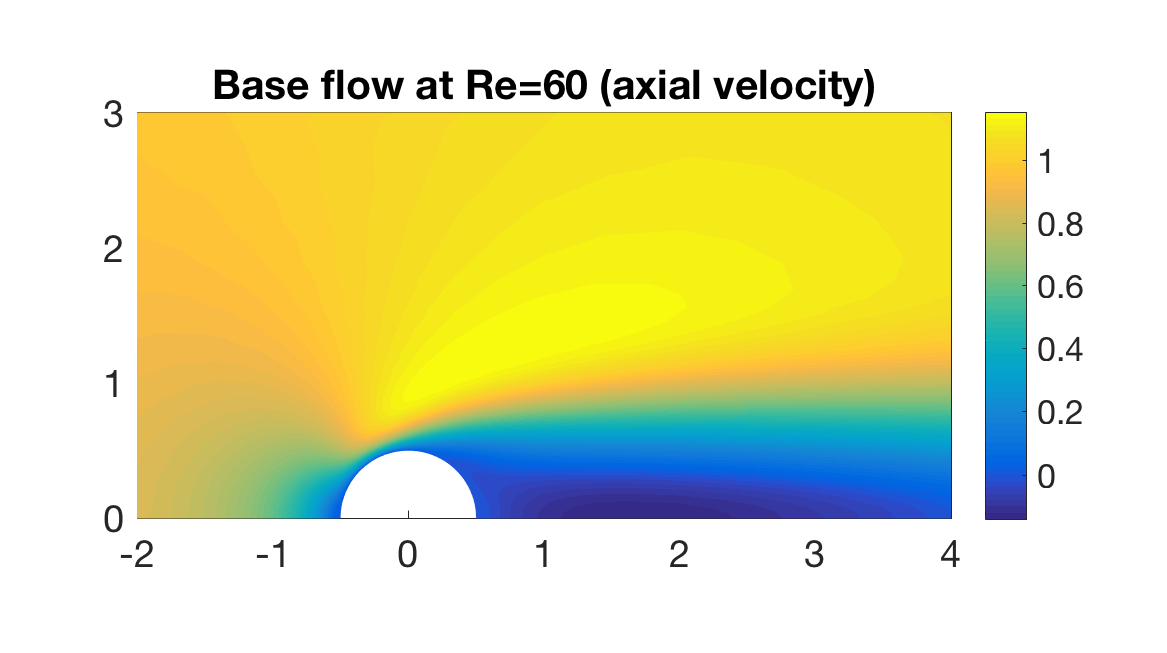
\includegraphics[width= \linewidth]{Cylinder_BaseFlowRe60.png}
\caption{Base flow for the flow over a cylinder at $Re=60$. Pressure field (color levels) and streamlines (iso-levels of the streamfunction $\psi$). }
\label{fig:Baseflow}
\end{figure}

\begin{figure}
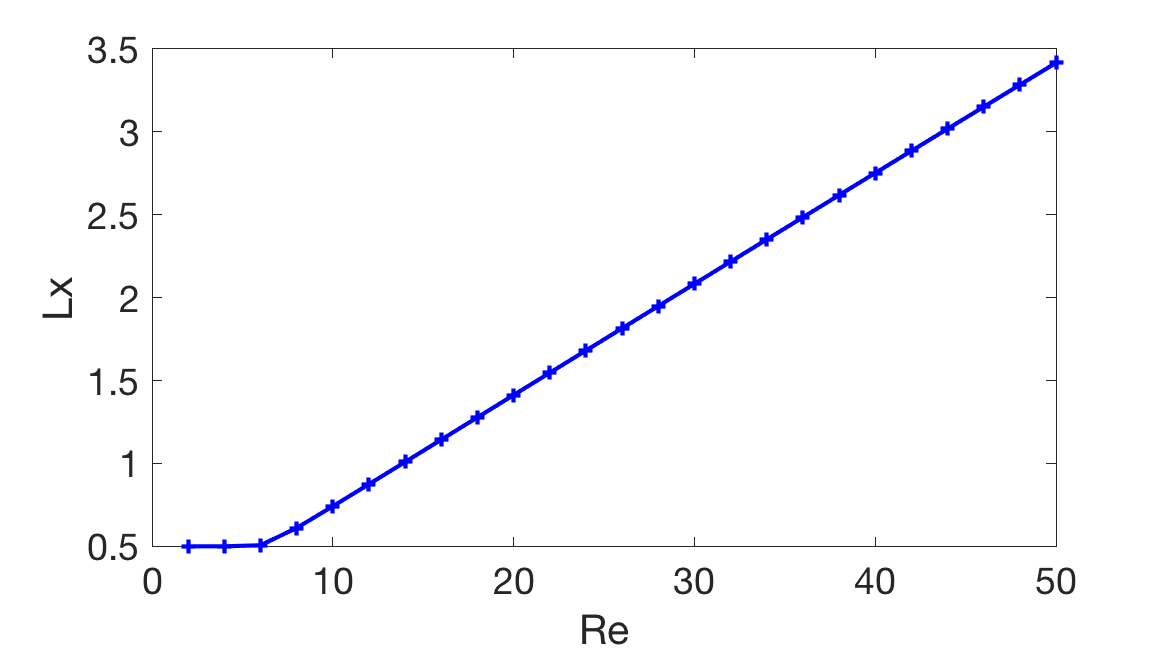
\includegraphics[width=\linewidth]{Cylinder_Lx_baseflow.png}
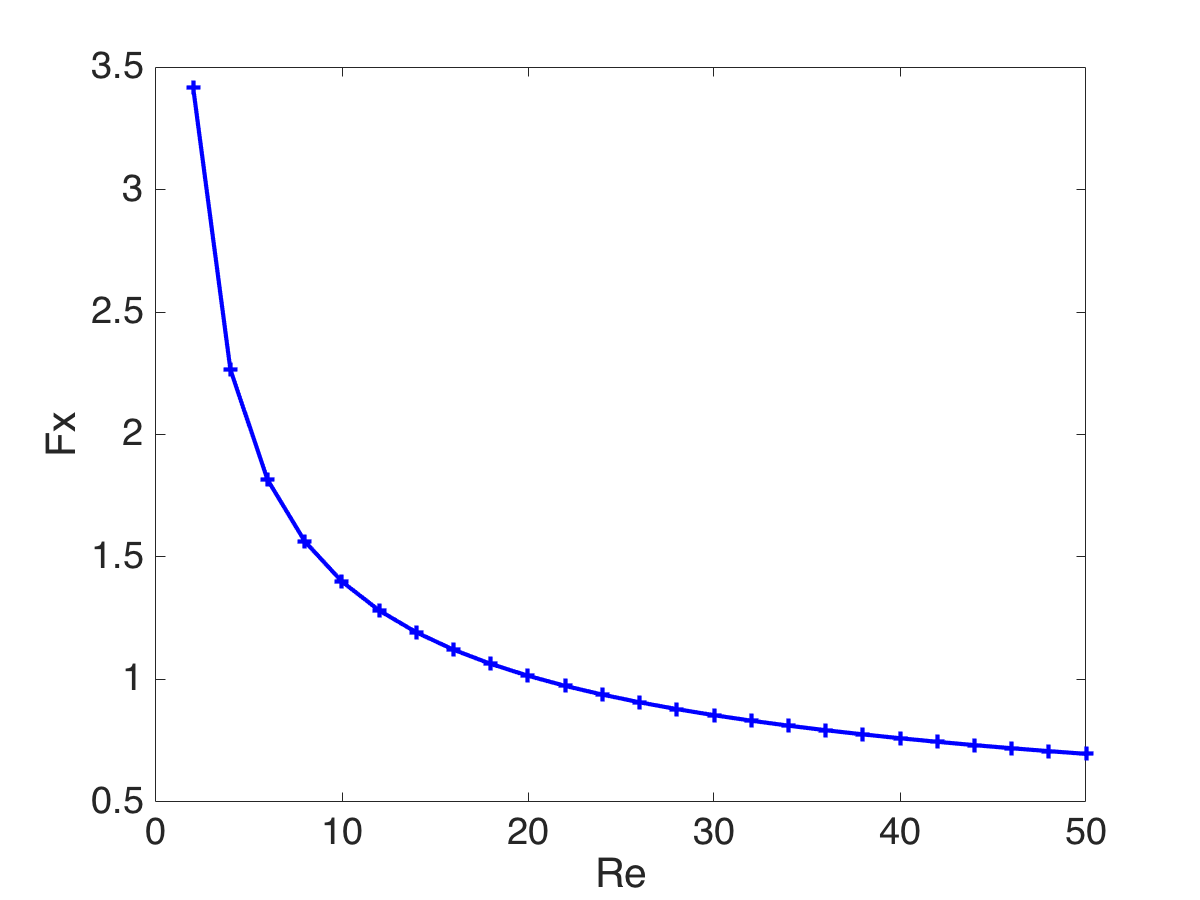
\includegraphics[width=\linewidth]{Cylinder_Fx_baseflow}
\caption{Recirculation length $L_x$ $(a)$  and nondimensional drag $F_x$ ($b$) of the base flow over a cylinder as function of $Re$.}
\label{fig:LxandDrag}
\end{figure}




\subsection{Mesh adaptation procedure}
\vspace{.2cm}

As for any numerical method, a crucial aspect for numerical efficiency is the design of the mesh. The finite element method allows using unstructured mesh and hence to have a local adaptation. %Following Sipp \& Lebedev, 
The most common procedure is to decompose the domain into several parts with different grid densities; for instance for the wake of a cylinder, we will design a near-wall region with very small  size, a wake region with intermediate mesh size, and an outer region with large mesh size. The drawback of such mesh generation guidelines is that the design relies on an a priori expectation of the regions where gradients will be large. 

In our implementation, we use an automated mesh adaptation method. %which provides an optimal mesh adapted to the structure of the flow. 
The implementation relies on the AdaptMesh procedure of the FreeFem++ software. This procedure is detailed in ref. \cite{adapt}. 
In short, the classical Delaunay-Voronoi algorithm produces a mesh with gridpoint distribution specified by a {\em Metric } matrix $\cal M$. The AdaptMesh algorithm consists in using as a metric the {\em Hessian} (second-order spatial derivatives) of an objective function $u_h$ defined over the domain, \textit{i.e.} ${\cal M} = \nabla \nabla u_h$. The precision can be controlled by specifying an objective value for the interpolation error of the function on the new mesh.

To build an optimal mesh for the base-flow calculation, the idea is to use as the objective function $u_h$ the solution ${\bf u}_b$ itself, as computed on a previous mesh. %The procedure thus ensures that the mesh will be locally adapted to the gradients of the base flow. 
The base flow is then recomputed on the adapted mesh, providing a better approximation of the solution. The procedure can be repeated over a few steps to ensure a right convergence.

%The mesh generated by the previous way may not be optimal for the stability calculations as the structure of the eigenmode may be more complex than that of the base flow.  To tackle this aspect, the idea is to subsequently adapt the mesh to both the mesh flow and the results of the stability calculation.This is easily done with FreeFem, as the  AdaptMesh procedure can be used with several objective functions.We have experimented four different strategies.The first (D strategy) is to adapt the mesh to the base flow and the structure of the leading direct eigenmode. A second strategy (A) is to use the adjoint mode instead of the direct mode for mesh adaptation. However, as the sensitivity of the eigenvalue to perturbations of the operator (including discretization errors) is more closely linked to structural sensitivity concepts, it sounds a better idea to use either the 'wavemaker' $S_w$ or the endogeneity $S_e$ to adapt the mesh, leading to the two last experimented strategies, called S and E.Note that using the S strategy was already experimented in {\em \cite{GiannettiLuchini} for the wake of a cylinder (IS THAT THE RIGHT REFERENCE ??}).Mesh adaptation using the scalar product of the direct and adjoint eigenmodes (which turns out to be equivalent to the E strategy introduced here considering the definition of the endogeneity) was also proposed in \cite{mavripilis2015adjoint}.A detailed comparison of the four strategies is reported in appendix A.It is shown that for the case of a cylinder, all strategies give the same values for base-flow drag, eigenvalues and several properties of the nonlinear limit cycle (see sec. 4) with less than $0.3\%$ deviation, but that the A, E and especially the S strategy lead to significantly lower number of grid points compared to the D strategy.
%The practical conclusions of this study are the following recommendations:

%\begin{itemize}
%\item[-] 
%First, if one is only interested in the eigenvalues --for instance to plot growth rates as function of Reynolds or to identify the critical Reynolds number,-- the A, E or S strategies are the best options. In the case of the cylinder, the S strategy leads to the lightest mesh. The E strategy results in a more refined mesh as the function $S_e$ is complex and displays more gradients than the real-valued function $S_w$ (as illustrated in figure \ref{fig:StructEndo}); hence the sensitivity revealed by the phase of $S_e$, which may be significant, is not captured by using the simpler function $S_w$. In the case of the flow around a cylinder,  this loss of information has no practical effect on the results, but for usage with more complex flows, our recommendation for future studies will be to favour the E strategy.
%\item[-] 
%The situation is different if one wants to design a mesh allowing to study the flow structure in the whole domain (for instance for plotting its structure). In that case, using A,E or S strategy will allow to accurately compute the eigenvalue and the structure of the mode in the wavemaker region, but will not allow for a proper resolution in the regions located far away where the direct mode may reach large amplitude. This is particularly the case for open flows characterized by large spatial convective amplifications. In such cases the D strategy is the only way to get a proper description of the eigenmode in the whole domain.
%\end{itemize}

The mesh generated in the previous way may not be optimal for the stability calculations as the structure of the eigenmode may be more complex than that of the base flow. To remedy with this, the idea is to subsequently adapt the mesh to both the mesh flow and the results of the stability calculation. This is easily done with FreeFem, as the  AdaptMesh procedure can be used with several objective functions. We have experimented four different strategies. The first (D strategy) is to adapt the mesh to the base flow and the structure of the leading direct eigenmode. A second strategy (A) is to use the adjoint mode instead of the direct mode for mesh adaptation. However, as the sensitivity of the eigenvalue to perturbations of the operator (including discretization errors) is more closely linked to structural sensitivity concepts, it sounds a better idea to use the "wavemaker" $S_w$ to adapt the mesh, leading to the last experimented strategy, called S. 
Mesh adaptation using the scalar product of the direct and adjoint eigenmodes  (called E-strategy) was also proposed in \cite{mavripilis2015adjoint} (this quantity has also beed discussed by \cite{marquet2015endogeneity}). A detailed comparison of the four strategies is reported in appendix A. It is shown that for the case of a cylinder, all strategies give the same values for base-flow drag, eigenvalues and several properties of the nonlinear limit cycle (see sec. 4) with less than $0,3\%$ deviation, but that the A, E and especially the S strategy lead to significantly lower number of grid points compared to the D strategy. 
Note that a valid alternative (not yet available in the StabFem  project) is offered by the Error Sensitivity to Refinement recently proposed by \cite{Luchini2017}. 




In our implementation, the whole process of mesh adaptation (including projection and recomputation of the base flow on the new mesh) is monitored using the Octave/Matlab driver {\sf  SF\_AdaptMesh.m} ; the kind of adaptation  (to base flow only (BF), or D, A, S , E strategies) is decided by the the nature of the objects given as input to this function. In the current implementation it is possible to adapt the mesh to as much as 8 fields of diverse nature (for instance, multiple eigenmodes along with their adjoint fields, harmonic-balance Fourier components, etc...)


\section{Illustration for the wake of a cylinder (incompressible case)}  
\vspace{.2cm}

\paragraph{Problem description}
Here, we consider the two-dimensional flow of an incompressible fluid of density $\rho$ past a circular cylinder. 
All flow quantities are normalized using the uniform incoming velocity $U_{\infty}$ and the cylinder diameter $D$, which are the characteristic velocity and length scales used for the definition of the Reynolds number $Re= U_{\infty} D / \nu$.
The origin of the Cartesian frame of reference is considered located on the cylinder axis, the x-axis is chosen to be parallel to the incoming free-stream velocity while the y-axis with the cross-stream velocity. The dimensions of the computational domain are the following: $-40 \le x/D \le 80$ and $0 \le y/D \le 40$ (boundary conditions and their implementation are detailed in appendix D).
Note that we take advantage of the symmetry properties of the problem to only solve it on the positive $y$ half-domain. 

The hydrodynamic loads can be obtained by integrating the stress tensor over the cylinder surface.
In particular, the hydrodynamic lift and drag forces read
\footnote{ Note that $F_x$ and $F_y$ are actually nondimensional forces per unit length. 
For a cylinder of diameter $D$ and length $L$ (assuming $L\gg D$ so that the assumption of 2D flow makes sense), 
the corresponding dimensional forces are $F_x^* = \rho U_\infty^2 D L F_x $ and $F_y^* = \rho U_\infty^2 D L F_y$. 
Alternatively, one may characterize the forces through the drag and lift coefficients $C_x$ and $C_y$. With the usual convention, 
The connection between the nondimensional forces and the force coefficients is $C_x = 2 F_x$ ; $Cy = 2 F_y$.
}
\be{drag}
F_x = {\cal D}_{Re} ({\bf u},p) \equiv 
  \int_{\Gamma_{cyl}} \left[-p {\bf n} + \frac{2}{Re} {\mathsf{D}}({\bf u}) \cdot {\bf n} \right]   \cdot {\bf e_x} d\ell,
\ee
\be{lift}
F_y = {\cal L}_{Re} ({\bf u},p) \equiv
  \int_{\Gamma_{cyl}} \left[-p {\bf n} + \frac{2}{Re} {\mathsf{D}}({\bf u}) \cdot {\bf n} \right]   \cdot {\bf e_y} d\ell. 
\ee
where $\Gamma_{cyl}$ is the boundary of the cylinder. %The factor 2 stands for the fact that our numerical domain is half the physical domain.


\paragraph{Mesh adaptation procedure}

Let us now consider the Octave/Matlab code reported in figure \ref{Listing2}. First we build an initial mesh (line 1), and compute base flow solutions for increasing values of the Reynolds number up to $Re = 60$ (lines 3-9).
Then we perform the mesh adaptation with S strategy, as explained previously (line 13).
The resulting mesh, depicted in figure \ref{fig:mesh2}, is used for the rest of the computations presented in this paper (except for plotting the structure of the direct eigenmode in figure \ref{fig:Eigenmode}$(a)$ and computing the energy of the nonlinear perturbation displayed in figure \ref{fig:HB_SC_DATA_COMP}$(d)$ which adopted a finer mesh obtained with the strategy D). 
Appendix A presents additional tests regarding mesh convergence, and demonstrates that results obtained with the resulting mesh are reliable within $0.3\%$ accuracy tolerance for the eigenvalue. It must be emphasized  that the mesh generated through this adaptation process is very light, with only 2048 vertices, which is significantly less than reported in previous works (for instance, in their mesh convergence studies, \cite{SippLebedev} and \cite{MLugo2014} used respectively 190868  and 6731 vertices).


%It is shown that as well as doing mesh adaptation with the eigenmode structure instead of the sensitivity, as discussed above, gives comparable results within $1\%$ as for the eigenvalue of the most amplified mode.







%The produced outputs (lines 14-17) gives information about the resulting mesh. 
%Note the values $h_{min}$ and $h_{max}$ of the smaller and larger edges, as well as the local grid size at four points A,B,C,D defined as $(x_A,y_A) = (0.5,0)$ (at the surface of the cylinder at the position of maximum shear), $(x_B,y_B) = (0.5,2.5)$ (at the location of the peak of structural sensitivity, see next section), $(x_C,y_C) = (0.,4)$ (in the near wake), and $(x_D,y_D) = (0.,10)$ (in the the far wake). Finally, the base flow is automatically recomputed on the resulting mesh (line 18-19). Finally, lines 21-22 plot the mesh and base flow structure, producing the result displayed in figure (\ref{fig:Baseflow}).

\paragraph{Base flow}

Having thus produced a convenient mesh, we can now illustrate the properties of the base flow as a function of Reynolds number. Figure \ref{Listing2} shows how to compute and plot with StabFem the two most commonly studied quantities, namely the recirculation length $Lx(Re)$, \textit{i.e.} the location of the stagnation point at the rear of the recirculation region, and the drag force $F_x(Re)$.
Note that the object \verb|bf| is defined as a structure with fields \verb|Fx| and \verb|Lx|. 
The resulting plots are given in figure \ref{fig:LxandDrag}, and are in good agreement with known results for this classical problem.
In particular, for low Reynolds, the recirculation $L_x(Re)$ is equal to $0.5$ (which is the radius of the cylinder) indicating the absence of a recirculation region. The latter appears for $Re > 4.8$, in accordance with known results.

An illustration of the structure of the base flow is given in figure \ref{fig:Baseflow},  for the case $Re = 60$. This figure is obtained using the Matlab/Octave function {\sf  SF\_Plot.m}, which is built over the function {\sf  ffpdeplot.m} developed by M. Meister and also distributed on an open-source basis
\footnote{\url{https://github.com/samplemaker/freefem\_matlab\_octave\_plot}}.  
This function provides a number of possibilities for plotting data on unstructured meshes, including color plots, isolevels, streamlines, quiver plots, etc\ldots
The choice of parameters used here (lines 8-10 of the script in figure \ref{Listing2})  allows plotting both the pressure field and selection of streamlines (through isocontours of the streamfunction $\psi$). This representation allows to easily visualize the extension of the recirculation region. In accordance with figure \ref{fig:LxandDrag}$(b)$, for $Re = 60$ the recirculation length is $L_x \approx 4.07$.





\begin{figure}
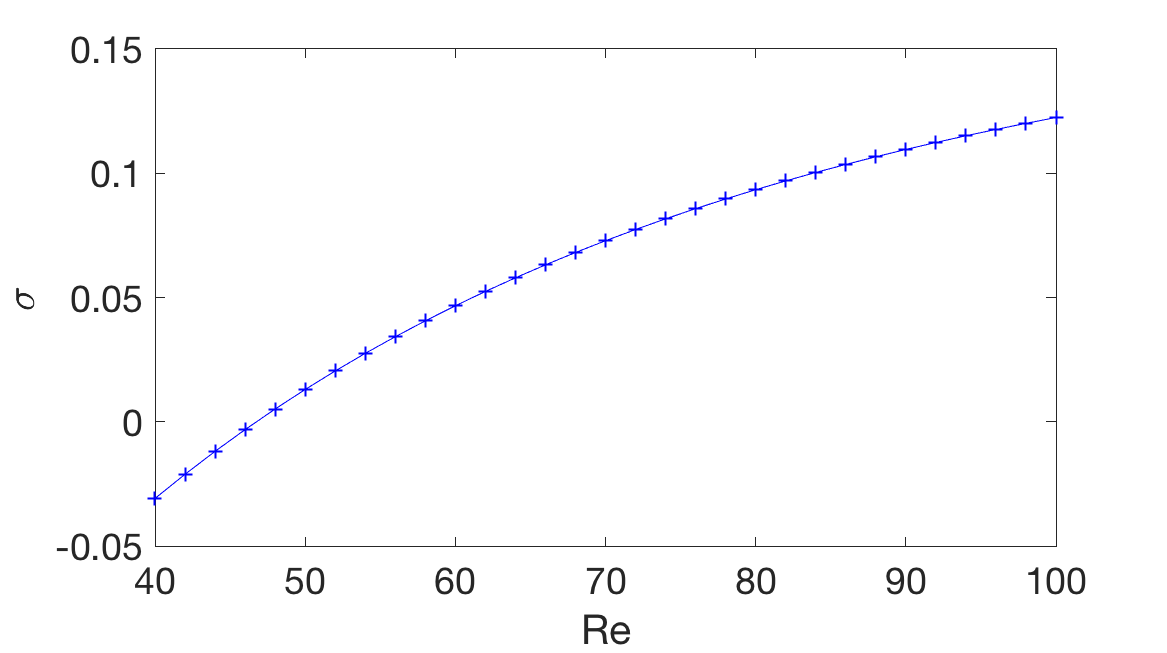
\includegraphics[width=\linewidth]{Cylinder_Sigma_Re.png}
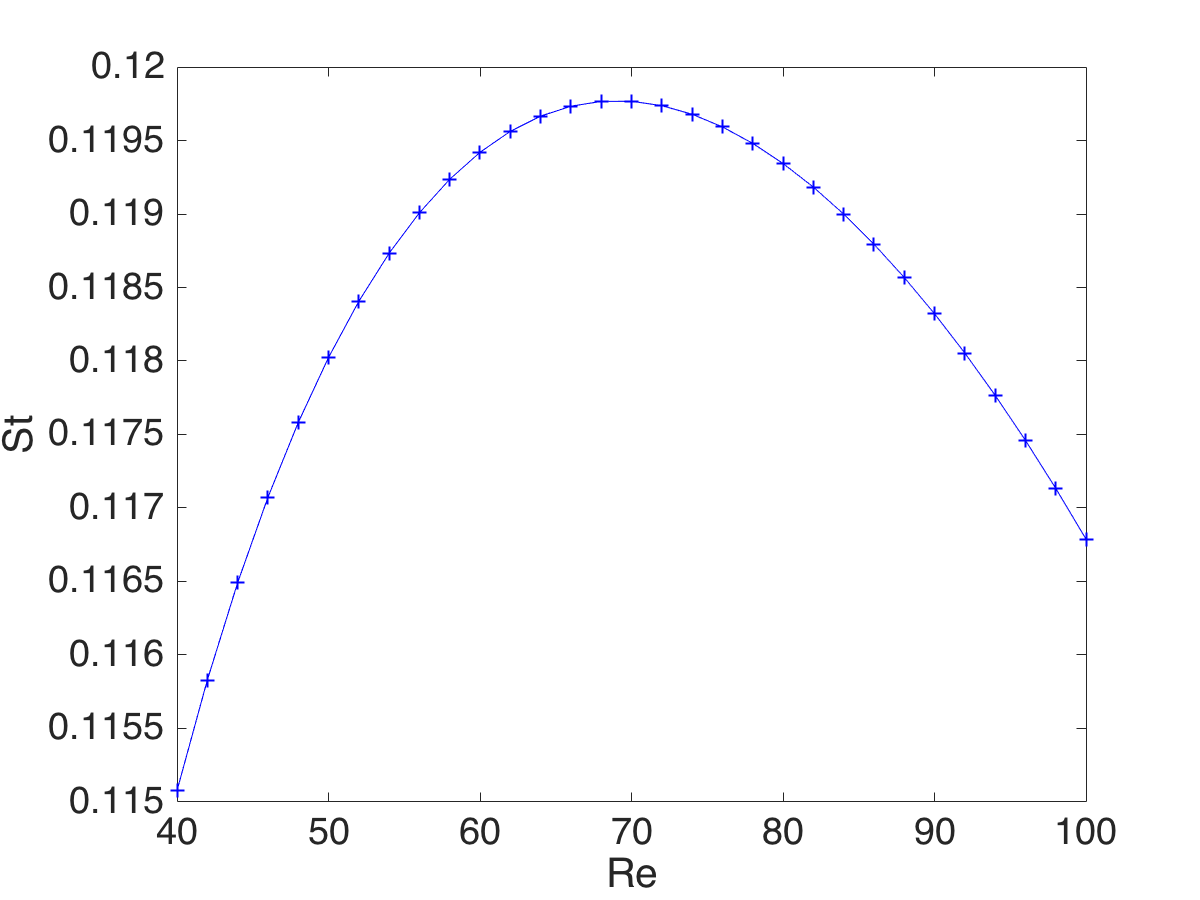
\includegraphics[width=\linewidth]{Cylinder_Strouhal_Re.png}
\caption{Growth rate $\sigma$ $(a)$  and Strouhal number $St = \omega/2\pi$ ($b$) as function of the Reynolds number.}
\label{fig:SigmaOmega}
\end{figure}

\begin{figure}
%\vspace{-.5cm}
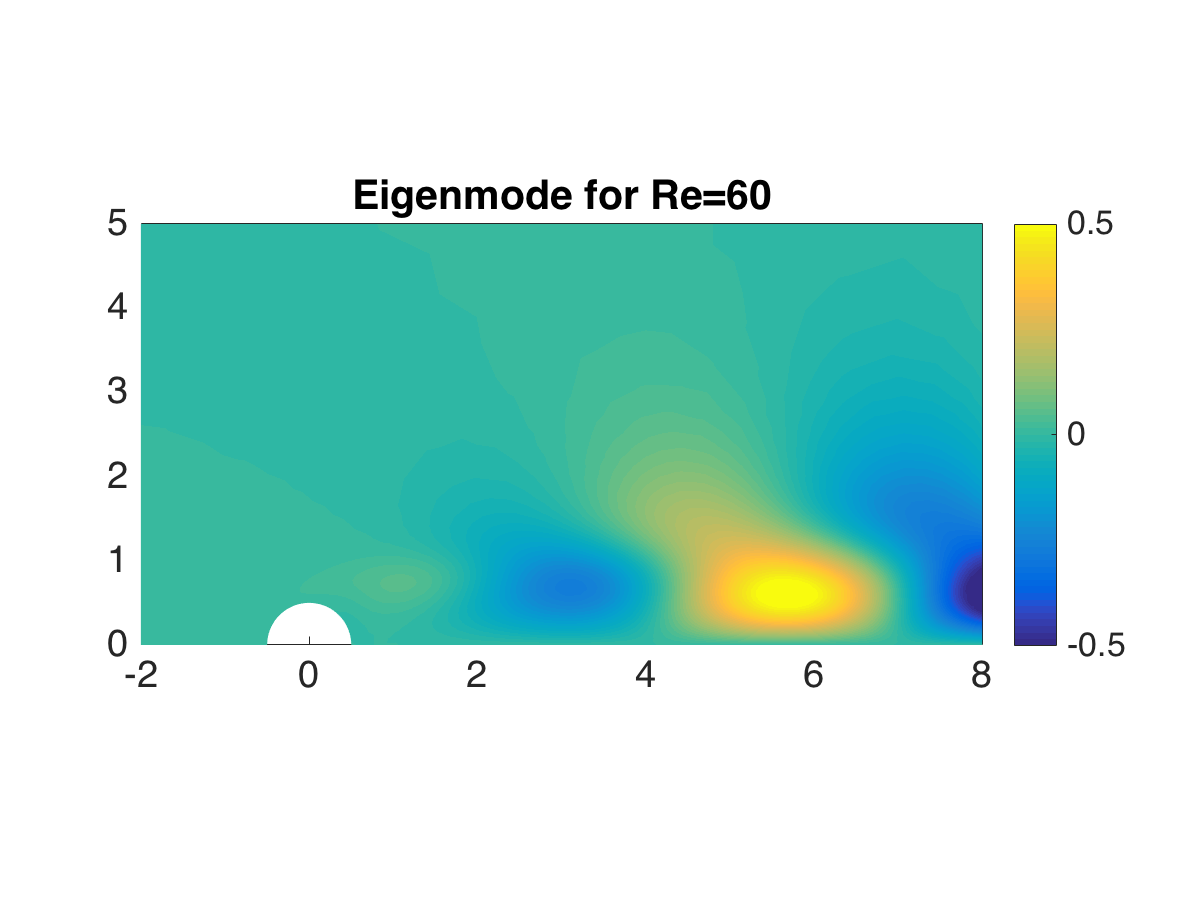
\includegraphics[width=\linewidth]{Cylinder_EigenModeRe60_AdaptS.png}%{Cylinder_EigenModeRe60_AdaptD.png}
%\vspace{-.5cm}
%\vspace{-.5cm}

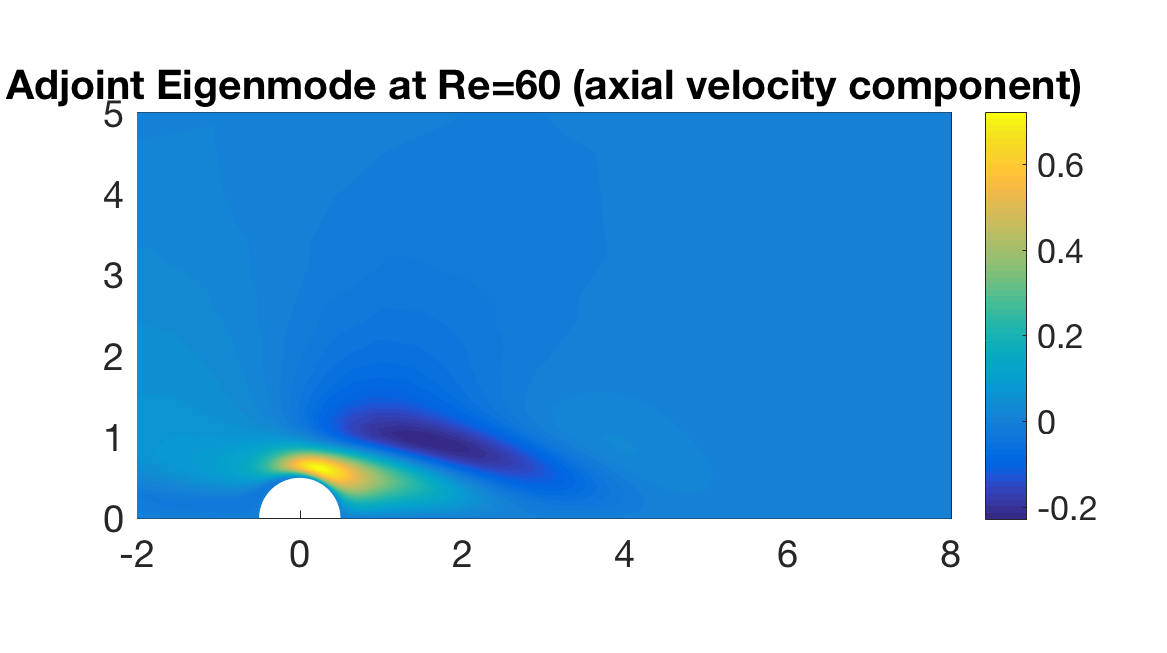
\includegraphics[width=\linewidth]{Cylinder_EigenModeAdjRe60.png}
%\vspace{-.5cm}\vspace{-.5cm}
%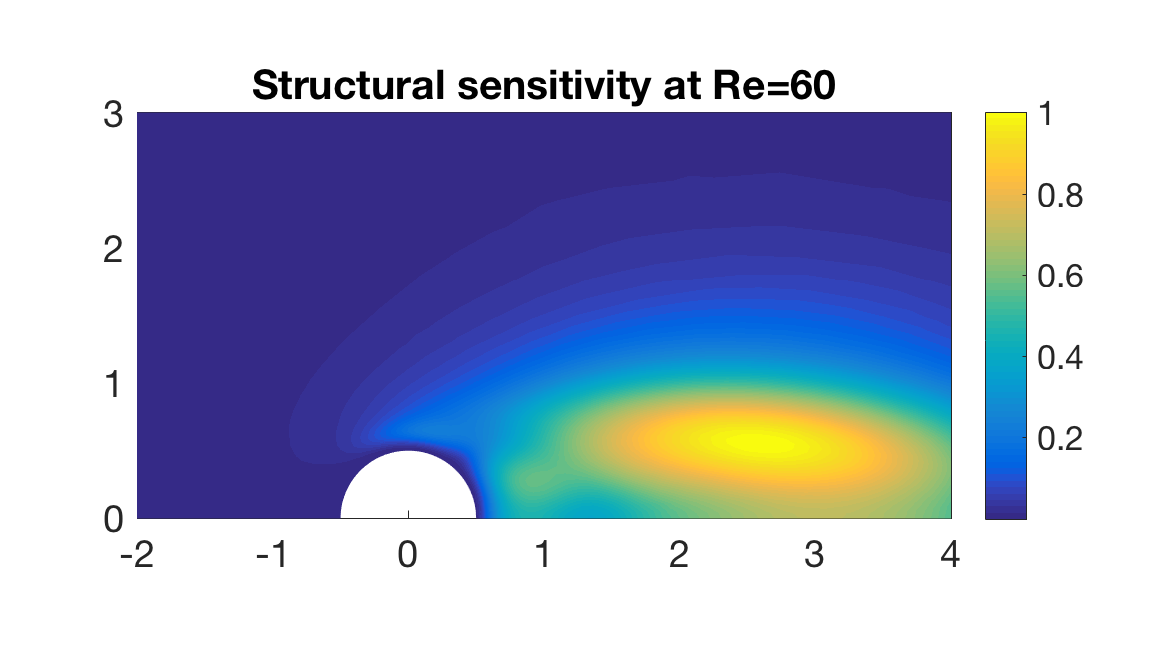
\includegraphics[width=\linewidth]{Cylinder_SensitivityRe60.png}
%\vspace{-.5cm}
\caption{Contour plot of the streamwise velocity component: $(a)$ (Direct) Eigenmode; $(b)$ Adjoint mode at $Re= 60$.}
\label{fig:Eigenmode}
\end{figure}

\begin{figure}
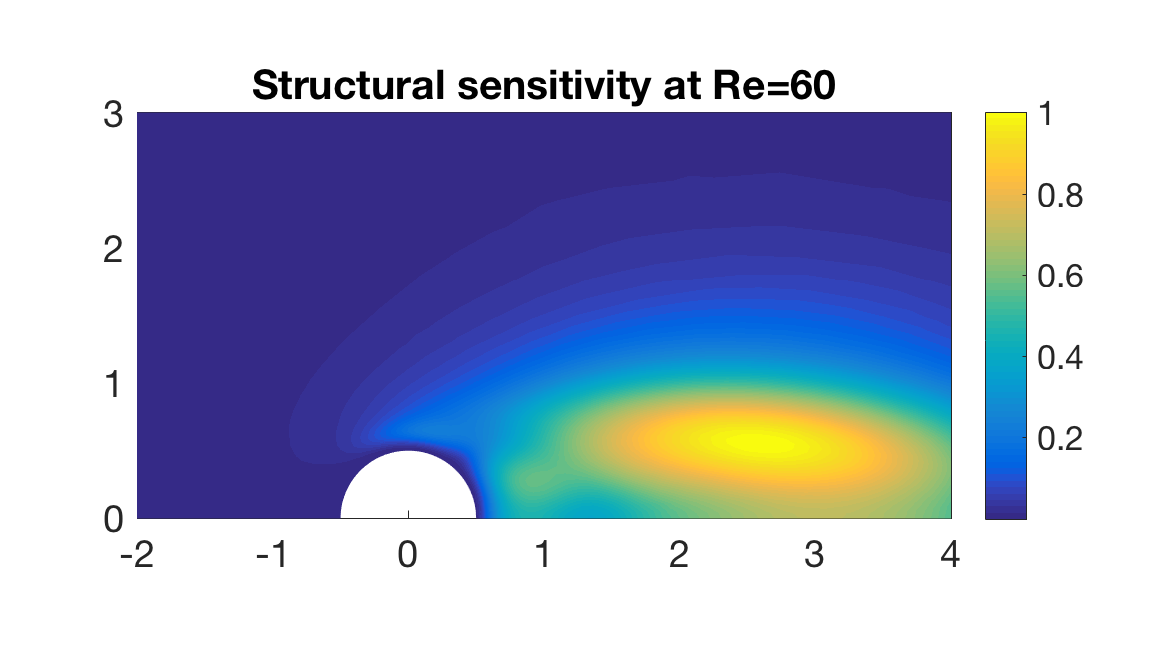
\includegraphics[width=\linewidth]{Cylinder_SensitivityRe60.png}
%\vspace{-.5cm}
\caption{ Structural sensitivity $S_w$ for the cylinder's wake at $Re= 60$. The red line represents the streamline bounding the recirculation region.}
\label{fig:StructEndo}
\end{figure}



%\begin{figure*}
%\small
%\begin{lstlisting}
%\end{lstlisting}
%\normalsize
%\caption{Illustration of the procedure to compute stability properties and adapt the mesh using StabFem (from script {\em SCRIPT\_CYLINDER.m}. }
%\label{listing4}
%\end{figure*}

\paragraph{Linear stability results}

We investigate the stability of the base flow field by performing a parametric study of the eigenproblem \eqref{LEP}. In this way, we determine the critical Reynolds number $Re_c$ from which the steady base flow first becomes unstable: to this end it is useful to remember that a flow state is linearly unstable when the real part of  the leading eigenvalue, \textit{i.e.} the growth rate, is positive. In our implementation, a parametric study is performed by looping over increasing Reynolds, corresponding to lines 21-30 of the script in figure \ref{Listing2}. Note that at line 26 the options {\sf  'shift, 'cont' ,'guess', em} transmitted to the driver {\sf  SF\_Stability} allow to use an optimum value for the shift interpolated using the previous computations, and a guess value to initialize the shift-invert procedure corresponding to the previously computed eigenmode. Both these ideas very efficiently accelerate the calculations (the shift-invert procedure typically converges after only 2-3 iterations).

Figure \ref{fig:SigmaOmega} shows growth rate and the Strouhal number $St=a\omega/2 \pi U_{\infty}$ as a function of the Reynolds number.
It is easy to check that the critical Reynolds number is about 47 for the first mode.
The associated direct eigenmode is depicted in figure \ref{fig:Eigenmode}.
The spatial structure of this mode extends downstream of the bluff body and is characterized by streamwise extended spatial disturbances.
On the other hand, the adjoint mode is highly localized near the cylinder on the upper (and lower) side of the body surface.
We recall that the adjoint field provides useful information about the mechanism to flow receptivity to momentum forcing and mass injection.
We note also that this receptivity decays rapidly both upstream and downstream of the bluff body.

The structural sensitivity $S_w$ introduced in section 2.2 is displayed in figure \ref{fig:StructEndo}. As discussed in section 2.2, both these quantities allow identifying the "active" flow regions responsible for the instability mechanism. The real quantity $S_w$ indicates that the most active region roughly coincides with the recirculation bubble. 
%The endogeneity $S_e$ yields more information. The sign of the real part (color levels)  indicate that the two most destabilizing regions are the boundary layer at the top of the cylinder and the shear layer bonding the recirculation region, and that the region of the stagnation point and the exterior of the recirculation region are destabilizing. The imaginary part (isolevels) indicate that the frequency selection occurs in the shear layer region.


\section{Extension : compressible flows}  
\label{sec:compressible}.

The main concepts of global linear stability analysis, exposed in section 2 for the case of incompressible flows, are directly generalizable to more complex situations involving compressibility, fluid-structure interactions, deformable free surfaces, etc... Such more complex situations can be studied using the same class of numerical methods and the same methodology. One of the ambitions of the StabFem software if to provide a unified procedure to perform such stability studies, so that despite the fact that the underlying equations may be different, the corresponding Octave/Matlab scripts will be almost the same in all cases. In this section, we will illustrate this point for the case of a compressible flow, keeping the geometry as a 2D cylinder, and will reproduce the results of the recent study of \cite{Fani2018}.

\subsection{Analysis and implementation}

In the compressible case, the Navier-Stokes equations have to be formulated in terms of a state-vector $[{\bf u},p,\rho,T]$ with larger dimension. 
The equations involve a larger number of terms but can be written in a compact way as follows :


\begin{eqnarray} \label{NSprimitive}
\partial_t {\cal B} [{\bf u},p,\rho,T] = {\cal NS}  [{\bf u},p,\rho,T] 
\end{eqnarray}

Here $\cal B$ is a "weight" operator specifying the coefficients in front of the time-derivatives of $[{\bf u},p,\rho,T]$ , and the operator $ {\cal NS}  [{\bf u},p,\rho,T] $ specifies the time-evolution of  $[{\bf u},\rho,T]$ coming from the momentum, energy and mass balances as well as the state equation linking $[p,T,\rho]$. The detailed form of these equation is given in \cite{Fani2018}. 

Starting with this form, the two main steps of the analysis, namely computation of a base-flow and eigenvalue computation, can be done in the same way as explained in sec. 2. Namely :
\begin{itemize}
\item[-] The base-flow $[{\bf u}_b,p_b,\rho_b,T_b]$ is the solution of ${\cal NS}  [{\bf u}_b,p_b,\rho_b,T_b]=0$ (eqs. 4$(a-d)$ of  \cite{Fani2018}) which can readily be computed using Newton iteration.
\item[-] Eigenvalues $\lambda$ and Eigenvalues $[\hat{{\bf u}},\hat{p},\hat{\rho},\hat{T}]$ are solutions of the eigenvalue problem $\lambda {\cal B}  [\hat{{\bf u}},\hat{p},\hat{\rho},\hat{T}]^T = {\cal LNS} [\hat{{\bf u}},\hat{p},\hat{\rho},\hat{T}]^T $ (eqs. 5$(a-d)$ of  \cite{Fani2018}) which can be solved using either single-mode shift-invert iteration or multiple-mode Arnoldi iteration.
\end{itemize}

In our implementation, these calculations are done by the FreeFem++ solvers {\sf  Newton2DComp.edp} and {\sf  Stab2DComp.edp}, which are quite different from their incompressible counterparts. However these solvers are wrapped by the same generic drivers {\sf  SF\_BaseFlow.m}  and {\sf  SF\_Stability.m}. The selection of which solver to use is made according to the parameters transmitted to them. 

\subsection{Example : 2D compressible flow around a cylinder}

 \begin{figure}
\includegraphics[width=\linewidth]{Cylinder_EigenmodeRe150Ma02_ux.png}
\caption{Structure of the unstable eigenmode (streamwise velocity component) for the compressible flow around a cylinder  $(Re= 150,M=0.2)$.}
\label{fig:compcyl_ux} 
\end{figure}


As an illustration, we consider the compressible flow around a 2D cylinder (same geometry as in previous section). The reader may find on the website of the project a script \footnote{ \url{https://gitlab.com/stabfem/StabFem/blob/master/STABLE_CASES/compCYLINDER/SRIPT_Fani.m}} reproducing the main results of the study of \cite{Fani2018}. We restrict here to the illustration of the structure of the unstable eigenmode for $Re = 150; M = 0.2$. Figure \ref{fig:compcyl_ux} shows the axial velocity associated to the eigenmode in a domain centered on the body. Figure \ref{fig:compcyl_p} displays the stucture of the pressure field on a much larger domain, allowing to detail the structure of the radiated acoustic field. The structure is in perfect agreement with the results of \cite{Fani2018} (see 5$(a)$ and $8$ of this paper). The value of the corresponding eigenvalue is also perfectly reproduced, namely $\lambda = 0.15273+0.64482i$.

 

 \begin{figure}
\includegraphics[width=\linewidth]{Cylinder_EigenmodeRe150Ma02_p.png}
\caption{Structure of the unstable eigenmode (pressure component) for the compressible flow around a cylinder  $(Re= 150,M=0.2)$. Upper half : real part ; lower half : imaginary part. }
\label{fig:compcyl_p}
\end{figure}

\section{Nonlinear global stability approaches}
\vspace{.2cm}
%\section{Computing the limit cycle for $Re>Re_c$ with Harmonic Balance}


%For $Re\right>Re_c$, the linear stability analysis based on the {\em base flow} does not allow to predict the properties of the limit cycle; in particular the Strouhal number is substantially underestimated. %It has been shown that investigating the stability properties of the {\em mean flow} obtained by averaging time-marching solution gives a better accordance. Attempts to on a rigourous basis  

In the past decade, efforts have been devoted to extend the range of validity of global approaches into the nonlinear regime for $Re>Re_c$, with the double objective of (i) describing the properties of the limit cycle reached after saturation and (ii) deriving amplitude equations describing the transient dynamics towards this cycle.
The two main milestones in this direction are the {\em weakly nonlinear model} (WNL) of Sipp \& Lebedev \cite{SippLebedev} and the {\em self-consistent model} (SC) of Manti\v{c}-Lugo et al. \cite{MLugo2014}.
In this review, we will only address the first of the two questions, namely  the description of the saturated cycle, and leave aside the question of transient dynamics. We will successively review the two aforementioned models, in a simplified formulation devoted to describe only the saturated cycle. We also provide a simple implementation of these two models. Finally, in line with the previous sections, this analysis is illustrated with results obtained for the wake of a cylinder.
  
 In this part, to simplify the notations, we symbolically write the Navier--Stokes equations as $\partial_t {\bf u} = {\cal NS} ({\bf u})$, therefore dropping the systematic reference to the incompressibility constraint and associated pressure field.
The same is done with the linearized operator ${\cal LNS}_{{\bf U}}( {\bf u})$. 

\subsection{General definitions in the nonlinear regime}

In the nonlinear regime, the {\em base flow} introduced in the linear theory is no longer relevant, especially when the oscillation amplitudes become large.
Instead, one may define a {\em mean flow} by using a time-average: 
%{\color{red} we taken the Reynolds decomposition ${\bf u}={\bf u}_m({\bf x})+{\bf u}'({\bf x},t)$, with ${\bf u}'$ the nonlinear perturbation and ${\bf u}_m$ the {\em mean flow} defined as the time-average  of the flow:}

\be{defumean}
{\bf u}_m({\bf x})  = \frac{1}{T} \int_0^{T}  {\bf u}({\bf x},t)  dt,
\ee
where $T = 2\pi/\omega$  is the period of the oscillation cycle. The difference between the instantaneous solution and the mean flow is then called the {\em nonlinear perturbation}, defined as 

\be{defuprime}
{\bf u}'({\bf x},t) =   {\bf u}({\bf x},t)-  {\bf u}_m({\bf x}).
\ee

A convenient measure of the unsteady part of the flow, which has been adopted in both the WNL and SC models, is the energy-amplitude, defined as the square-root of the total energy associated to the nonlinear perturbation:
\be{defAnergy}
A_E = \sqrt{\frac{1}{T} \int_0^{T} \left( \int_\Omega | {\bf u}' |^2 \, dS \right) dt}.
\ee

In the next sections we will document the predictions of the WNL and SC models regarding the quantities $A_E$ and $L_x$ adopted in past studies.
In addition, we will document two other quantities of practical interest: the Drag and Lift forces $F_x$ and $F_y$ exerted on the cylinder. 
Both are periodic functions of time and, owing to symmetry consideration, the drag contains only even harmonics and the lift only odd harmonics:

%\be{drag_lift_def}
%\begin{cases}
%F_x=F_{x,0} + \sum_{n=1}^\infty \big( F_{x,2n,c} \cos ( 2 n \omega t) + F_{x,2n,s} \sin( 2 n  \omega t ) \big) \\
%\begin{split}
%F_y  =  \sum_{n=1}^\infty \big(  F_{y,{2n-1},c} \cos ((2n-1) \omega t ) +\\
% F_{y,(2n-1),s} \sin ((2n-1) \omega t) \big)
%\end{split}
%\end{cases}.
%\ee
\begin{align}
F_x &=F_{x,0} + \sum_{n=1}^\infty \big( F_{x,2n,c} \cos ( 2 n \omega t) + F_{x,2n,s} \sin( 2 n  \omega t ) \big),
\\
\begin{split}
F_y  & =\sum_{n=1}^\infty \big( F_{y,{2n-1},c} \cos ((2n-1) \omega t )\\
             &\qquad + F_{y,(2n-1),s}  \sin ((2n-1) \omega t) \big).
\end{split}
\label{drag_lift_def}
\end{align}



In the sequel we will focus on the {\em mean drag}  $F_{x,0}$ and on the fundamental components of the lift  
$F_{y,1,c}$ and $F_{y,1,s}$. These quantities are easily retrievable from a numerical simulation or an experiment, and we will show how they can be predicted from the nonlinear global approaches.
 
  

   
%MThe mean drag is given by 

%$$F_{x,m} = D(u_m)$$
%with "Drag" operator defined in equation ().

%The oscillating lift $F_y(t)$  is a	 periodic function of period $T$, and we will 
%$$F_y = F_y,c


%The first milestone in this direction is the work of Sipp \& Lebedev \cite{SippLebedev} who used a weakly nonlinear development in terms of the distance to the threshold $Re-Re_c$. However, although derived on rigorous grounds, the weakly nonlinear development has a very limited range of validity and already fails for $(Re-Re_c) \approx 1$.
%More recently,  Manti\v{c}-Lugo et al \cite{MLugo2014} proposed an alternative approach termed {\em Self-consistent model} which succeeds in predicting the dynamics up to $Re =120$ and more. 
%This model was build as a linear stability approach build on a {\em mean flow} which includes a retroaction of the eigenmode. However, if one is interested in the limit cycle and not the transient,
%the approach is actually equivalent to a Fourier series decomposition of the flow with respect to time (an approach also known as {\em harmonic balance}) retaining only the two first terms. 
%The approach is based on a generalisation of the eigenmode ansatz \ref{} and 

%In the next sections, we thus successively present the weakly nonlinear model, the self-consistent model, and propose a direct resolution method for this latter model. 


%The relation with the initial method of Mantic-Lugo et al. will be discussed afterwards.

\subsection{The weakly nonlinear model}

%\paragraph{Analysis}


\begin{figure*}
\small
\lstinputlisting{SCRIPT_CYLINDER_Part2.m}
 \normalsize
\caption{Illustration of the procedure for nonlinear calculations using StabFem (extract from script {{\em SCRIPT\_CYLINDER\_ALLFIGURES.m})}. }
\label{fig:listingNL}
\end{figure*}



We first review the weakly nonlinear model of Sipp \& 
Lebedev\cite{SippLebedev}, also discussed by Gallaire et al. \cite{FDR2016}.  
The initial derivation of \cite{SippLebedev} makes use of a multiple scales method in order to obtain an amplitude equation.
This complete analysis is reproduced in appendix B. In the present paragraph, we give a simplified derivation of this model restricted to the description of the periodic saturated cycle.
The starting point can be taken as the following expansion of the velocity flow field:
\be{WNL1}
\begin{aligned}
&{\bf u} = {}  {\bf u}_{bc} + \epsilon \left[ A_{wnl}  \hat{\bf u} e^{i (\omega_c+\epsilon^2 \omega_\epsilon)  t} + c.c. \right]\\
&+ \epsilon^2 \left[ {\bf u}_\epsilon + |A_{wnl}|^2  {\bf u}_{2,0} + \left(  A_{wnl}^2 {\bf u}_{2,2} e^{2 i(\omega_c+\epsilon^2 \omega_\epsilon)  t} + c.c. \right) \right]\\
& + {\cal O}( \epsilon ^3),
\end{aligned}
\ee



This expansion is built as an asymptotic expansion in terms of the small parameter $\epsilon = \sqrt{1/Re_c - 1/Re}$ corresponding to the distance to the critical Reynolds number. 
The zero-order term ${\bf u}_{bc}$ is the base flow at the threshold $Re_c$.

In the first-order term, $\hat{\bf u}$ is the neutral eigenmode at $Re_c$ conveniently normalized (see discussion in appendix B), 
$A_{wnl}$ an amplitude which can be assumed as real, $\omega_c$ the frequency predicted by the linear approach at $Re=Re_c$ and $\omega_\epsilon$ a small deviation on the frequency. 

The second-order term contains three contributions: ${\bf u}_{\epsilon}$ is the modification to the base flow related to the increase of $Re$, ${\bf u}_{2,0}$ represents the nonlinear interaction of $\hat{\bf u}$ with its conjugate, ${\bf u}_{2,2}$ the nonlinear interaction of $\hat{\bf u}$ with itself.
These three terms are computed as solutions of nonsingular linear systems (see eqs. \eqref{eq:LL1}, \eqref{eq:LL2} and \eqref{eq:LL3} in appendix B).

At ${\cal O}( \epsilon ^3)$, compatibility conditions need to be enforced to ensure that the problem is correctly posed.
These conditions lead to an {\em amplitude equation} which relates the amplitude $ A_{wnl}$ to three parameters $\Lambda, \nu_{0}$ and $\nu_{2}$ which depend
uniquely on ${\bf u}_\epsilon$, ${\bf u}_{2,0}$ and ${\bf u}_{2,2}$, respectively (see equations \eqref{LAMBDA}, \eqref{NU0} and \eqref{NU2} in appendix B). Restricting to the description of the limit cycle, the {\em amplitude equation} takes the form:

\be{WNL3}
i \omega_\epsilon A_{wnl} = \Lambda A_{wnl} - (\nu_0+\nu_2)  |A_{wnl}|^2 A_{wnl}.
\ee


%where the coefficients $\Lambda$, $\nu_0$ and $\nu_2$ are given by We note that $\Lambda$ does not depend on the normalization choice of the eigenmode, discussed later, while $\nu_0$ and $\nu_2$ depend. 
The amplitude $A_{wnl}$ and the correction to the frequency are then determined by considering the real and imaginary parts of this equation, leading to
%\be{AWNL}
$
A_{wnl}= \sqrt{ \frac{\Lambda_r}{\nu_{0,r}+\nu_{2,r}}}
$ and
%\ee
%\be{omegaeps}
$
\omega_\epsilon = \Lambda_i- \Lambda_r \frac{\nu_{0,i}+\nu_{2,i}}{\nu_{0,r}+\nu_{2,r}} 
$
%\ee
where the subscripts $r$ and $i$ represent the real and imaginary parts.
Reintroducing the scaling, the  amplitude $A =  \epsilon A_{wnl} $ and the frequency $\omega$ of the limit cycle are thus predicted as
\be{ANL} 
A =  \epsilon A_{wnl} =\sqrt{ \frac{\Lambda_r}{\nu_{0,r}+\nu_{2,r} }} \sqrt{\frac{1}{Re_c}-\frac{1}{Re}},
\ee
\be{omegaWNL} 
\omega \equiv \omega^{(wnl)} =\omega_c+ \left( \Lambda_i- \Lambda_r \frac{\nu_{0,i}+\nu_{2,i}}{\nu_{0,r}+\nu_{2,r}} \right) \left(\frac{1}{Re_c}-\frac{1}{Re}\right)
\ee 


Finally, as specified above, we explain how the mean drag $F_{x,0}$ and fundamental components $(F_{y,1,c},F_{y,1,s})$ of the oscillating lift can be predicted by the WNL approach.
The mean drag  can be obtained by $F_{x,0} = {\cal D}_{Re}({\bf u}_m,p_m)$, where ${\cal D}$ is the drag operator defined in \eqref{drag} and 
$[{\bf u}_m,p_m]$ is the {\em mean flow}  
which corresponds to the time-average of expansion  \eqref{WNL1}, namely:
$
[{\bf u}_m,p_m] = [{\bf u}_{bc},p_{bc}] +\epsilon^2 \left( [{\bf u}_\epsilon,p_\epsilon] + A_{wnl}^2 [{\bf u}_{2,0}, p_{2,0} ] \right).
$
Developing the terms as an asymptotic expansion leads to:
\be{drag_cos}
 F_{x,0}(Re) \approx F_{x,0,{Re_c}} +  F_{x,0,\epsilon} \left(\frac{1}{Re_c}-\frac{1}{Re}\right)
\ee 
\begin{equation*}
\begin{aligned}
& \mbox{with} \quad F_{x0,{Re_c}}  = {\cal D}_{Re_c} ({\bf u}_{bc},p_{bc}), \quad \mbox{and}  
\\ 
& F_{x0,\epsilon} = {\cal D}_{Re_c} ({\bf u}_\epsilon, p_\epsilon ) - {\cal D}_{1} ({\bf u}_{bc},0) 
+ A_{wnl}^2 {\cal D}_{Re_c} ({\bf u}_{2,0},p_{2,0}). 
\end{aligned}
\end{equation*}
%_{\epsilon},p_\epsilon)
%D({\bf u}_{\epsilon})- 2\int_{\Gamma_{cyl}}} \mathbf{D} ({\bf u}_{bc}) \cdot {\bf n}  \cdot {\bf e}_x d \ell \right) 
%\\
%&+|A|^2 D({\bf u}_{2,0})\\
%&+2|A|^2\big(F_{x,r}({\bf u}_{2,2})\cos(2\omega t)
%-F_{x,i}({\bf u}_{2,2})\sin(2\omega t) \big),

Similarly the required components of the lift force are obtained by applying the lift operator ${\cal L}$ defined in \eqref{lift} 
to the order-one component of the expansion, leading to:
\be{lift_cos}
F_{y,1,c} - i F_{y,1,s} = 2 A_{wnl} {\cal{L}}_{Re_c}( {\bf \hat{u}},\hat{p} ) \sqrt{\frac{1}{Re_c}-\frac{1}{Re}}.
%|A|_i F_{x,i}({\bf \hat{u}})\sin(\omega t) \big),\\
%\end{aligned}
\ee

%\be{lift_cos}
%\begin{aligned}
%F_{y,WNL} =2\big(|A|_r F_{x,r}({\bf \hat{u}})\cos(\omega t)-
%|A|_i F_{x,i}({\bf \hat{u}})\sin(\omega t) \big),\\
%\end{aligned}
%\ee

%where $F_{x}$ and $F_{y}$ are given by and \ref{lift} (with the associated pressure field implicit), respectively . All terms in these equations can be matched with the interesting ones in \ref{drag_lift_def}: $F_{x,0}$ is the first 4 terms of \ref{drag_cos}; $F_{x,2,c}$, $F_{x,2,s}$ are the fifth and sixth terms of \ref{drag_cos}; $F_{y,1,c}$, $F_{y,1,s}$ are the first and second terms of \ref{lift_cos}. We note that the \textit{sin} term is associated to the phase of the forces in a physical way. }

%\iffalse
%\begin{eqnarray}
%\begin{aligned}
%F_{x,WNL} = F_{x}({\bf q}_{bc})&+\epsilon^2 \big( 
%F_{x}({\bf q}_{\epsilon})- 2\mathsf{D}({\bf u}_{bc}) \big)\\
%&+F_{x}({\bf q}_{2,0})|A|^2\\
%&+2F_{x,r}({\bf q}_{2,2}\cos(2\omega t)+
%2F_{x,i}({\bf q}_{2,2}\sin(2\omega t)
%),\\
%\end{aligned}\\
%F_{y,WNL} = |A|^2 \big[ F_{y}({\bf \hat{q}})e^{i\omega_{LC} t} +c.c. \big],
%\end{eqnarray}
%\fi


\paragraph{Implementation and results for the cylinder}




Lines 1-8 of the script shown in figure \ref{fig:listingNL} (extracted from the script 
{\sf SCRIPT\_CYLINDER\_ALLFIGURES.m}) illustrate the sequence of commands to 
perform the weakly nonlinear study for the cylinder wake.
On line 2, we first determine the instability threshold, and the corresponding base flow and eigenmode\footnote{This routine uses Newton iteration to directly compute the base flow, the eigenmode, the frequency and the critical Reynolds. The algorithm is very similar to the one presented for the HB, with an additional unknown (Re) and an additional constraint (normalization of the mode). The interested reader should reconstruct easily the whole procedure from the code provided.}. 
On line 3 we solve the adjoint problem required for some terms in the WNL formulation.
On line 4, we then compute all the terms and coefficients of the WNL model.
Lines 6-8 then process the results in a way they can be plotted.
%{\color{red}The other lines are explained latter.}
%After that, 
%we construct  vectors to store the frequency and the amplitude of the limit cycle in the 
%range $Re = [47.5-100]$. Note that for the computation at $Re=47.5$, we need a guess 
%for the amplitude, which is deduced from the weakly nonlinear approach on line 9. In 
%the sequel of the loop no guess value is prescribed, hence the solver uses 
%continuation.

%{\color{red} 
%The forces coefficients given by $F_x({\bf u})$ and $F_y({\bf u})$ are then converted in a more traditional form, $C_x=2F_x({\bf u})$ and $C_y=2F_y({\bf u})$.
%}



Figure \ref{fig:HB_SC_DATA_COMP} shows the predictions of the WNL approach regarding the frequency (expressed as a Strouhal number through $St = \omega/2\pi$), mean drag, amplitude of the oscillating lift, and energy-amplitude.
As discussed in \cite{SippLebedev} and \cite{FDR2016}, when compared to DNS results, this approach gives good prediction in the immediate vicinity of $Re_c$, but deviation appears very rapidly and disagreement is already large at $Re=48$ (although, as discussed by \cite{FDR2016} and also observed by \cite{Tchoufag2015}, a convenient definition of $\epsilon$ improves the prediction). 
These aspects are justified by the perturbative nature of the WNL approach. The description of the limit cycle can be extended to larger $Re$ with the approach presented next.  

\begin{figure}
\begin{center}
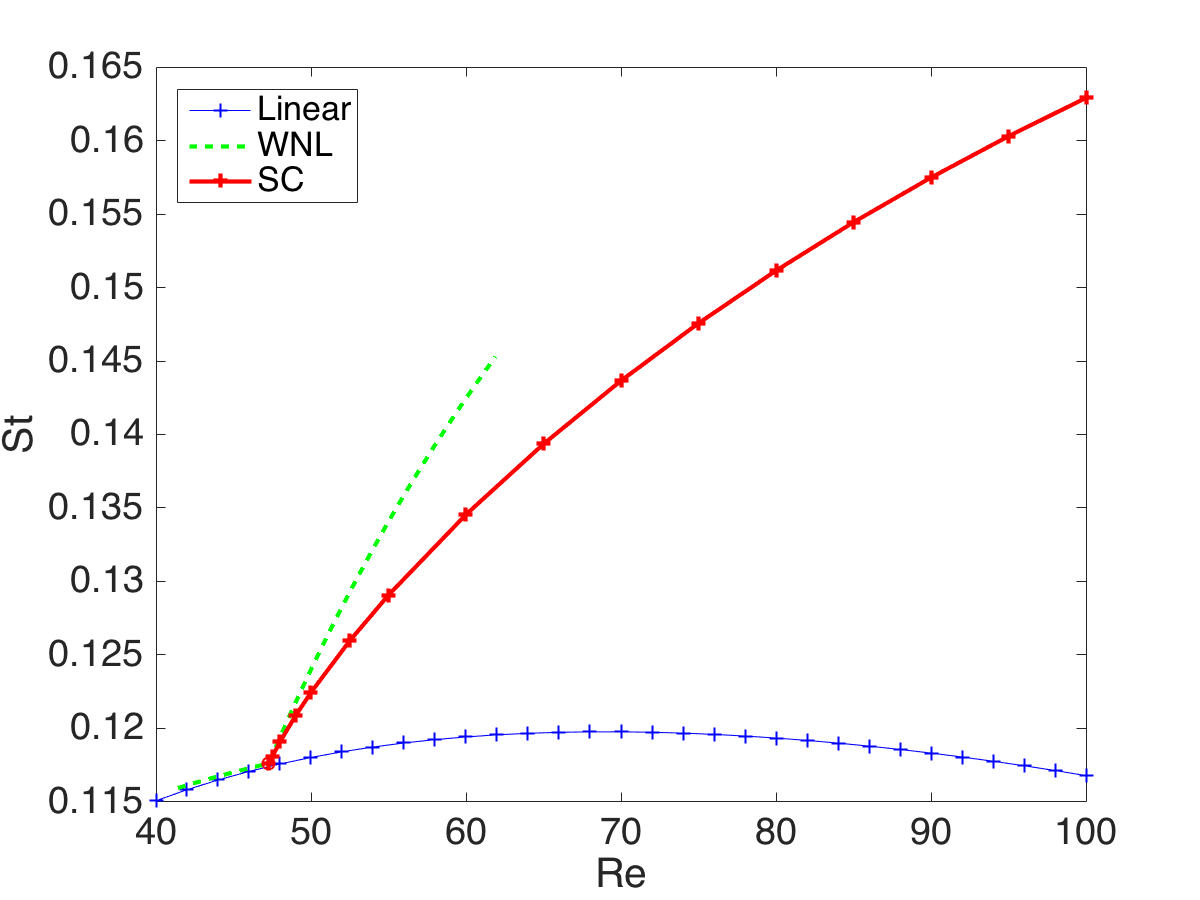
\includegraphics[width=0.9\linewidth]{Cylinder_Strouhal_Re_HB.png}
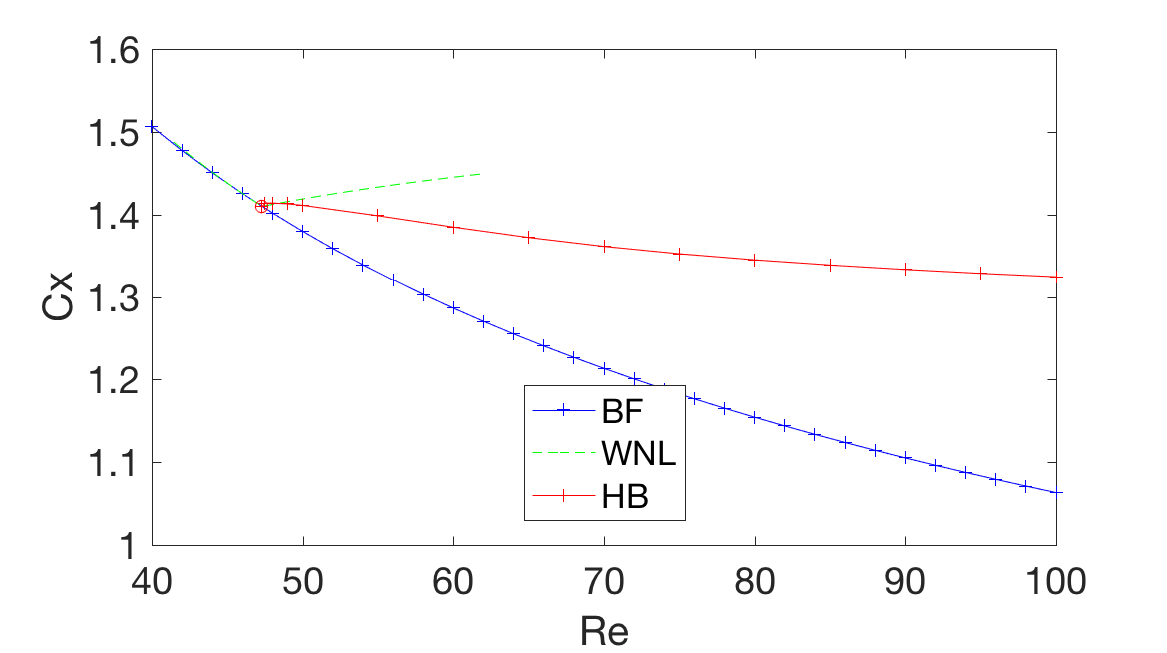
\includegraphics[width=0.9\linewidth]{Cylinder_Cx_Re_HB.png}
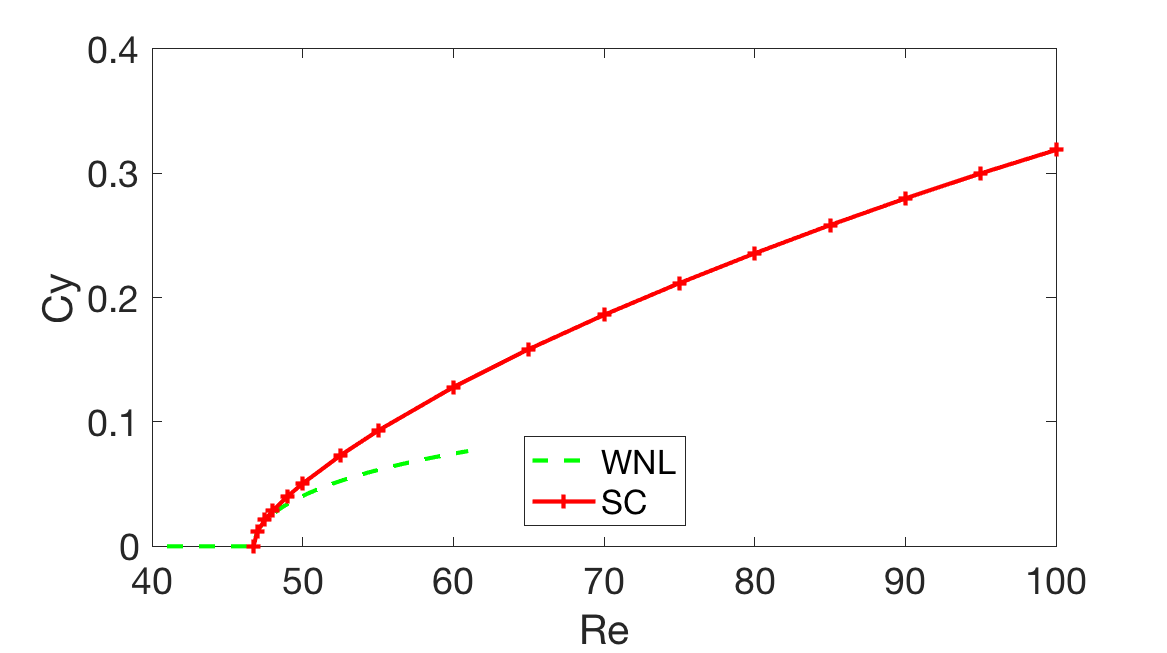
\includegraphics[width=0.9\linewidth]{Cylinder_Cy_Re_SC.png}
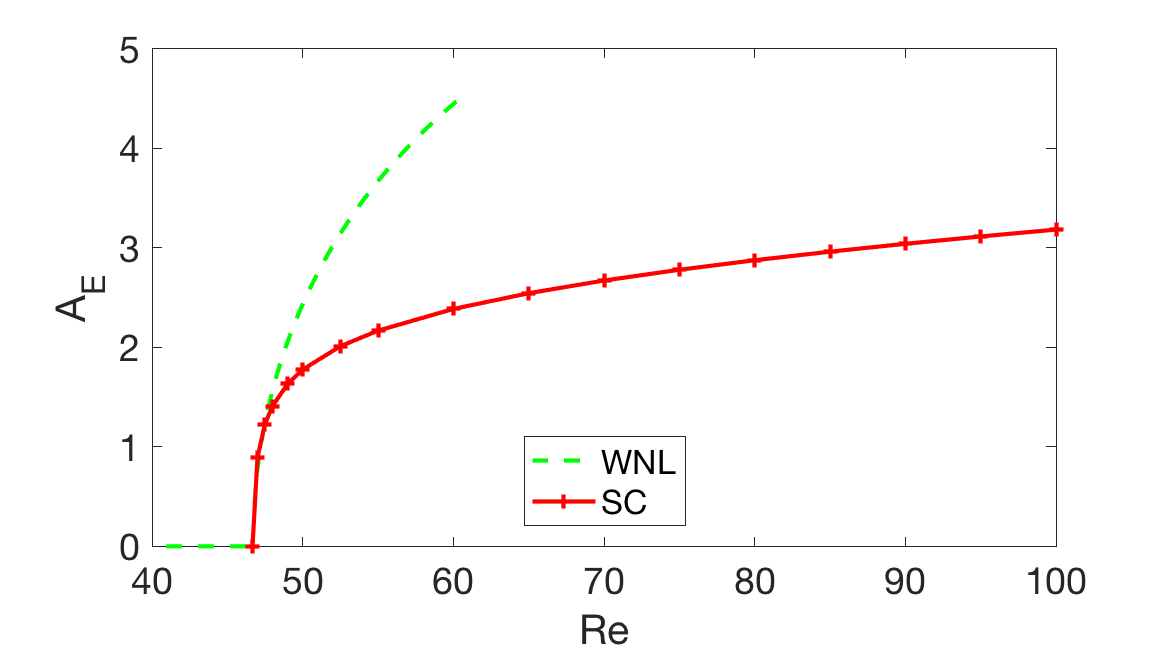
\includegraphics[width=0.9\linewidth]{Cylinder_Energy_Re_SC_AdaptD.png}
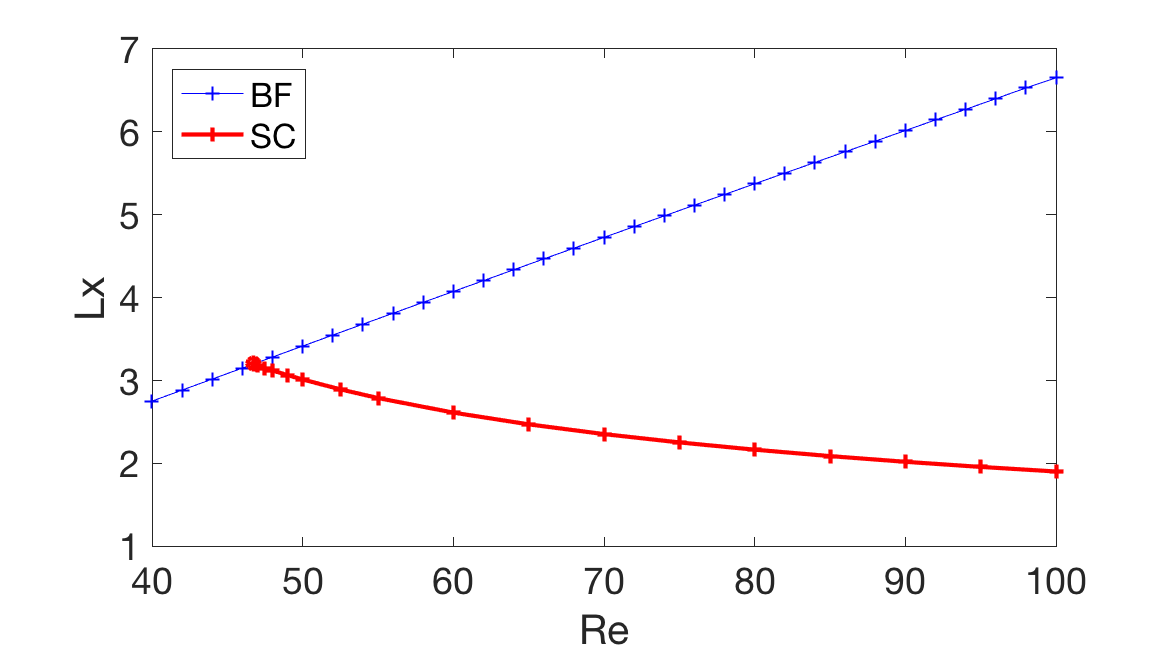
\includegraphics[width=0.9\linewidth]{Cylinder_Lx_Re_HB.png}
\end{center}
\caption{Comparison between the weakly nonlinear results (WNL), the harmonic balance data (HB1), and baseflow/linear results: Strouhal number $(a)$, Mean drag $(b)$, amplitude of oscillating lift $(c)$, Energy-amplitude of the nonlinear perturbation $(d)$ and recirculation length of mean/base flows $(e)$. 
%c_x should be consistent with the drag definition given at beginning
}
\label{fig:HB_SC_DATA_COMP}
\end{figure}



\subsection{The Self-Consistent model reformulated in the Harmonic-Balance formalism }
\paragraph{Analysis}

%\begin{figure}
%\begin{center}
%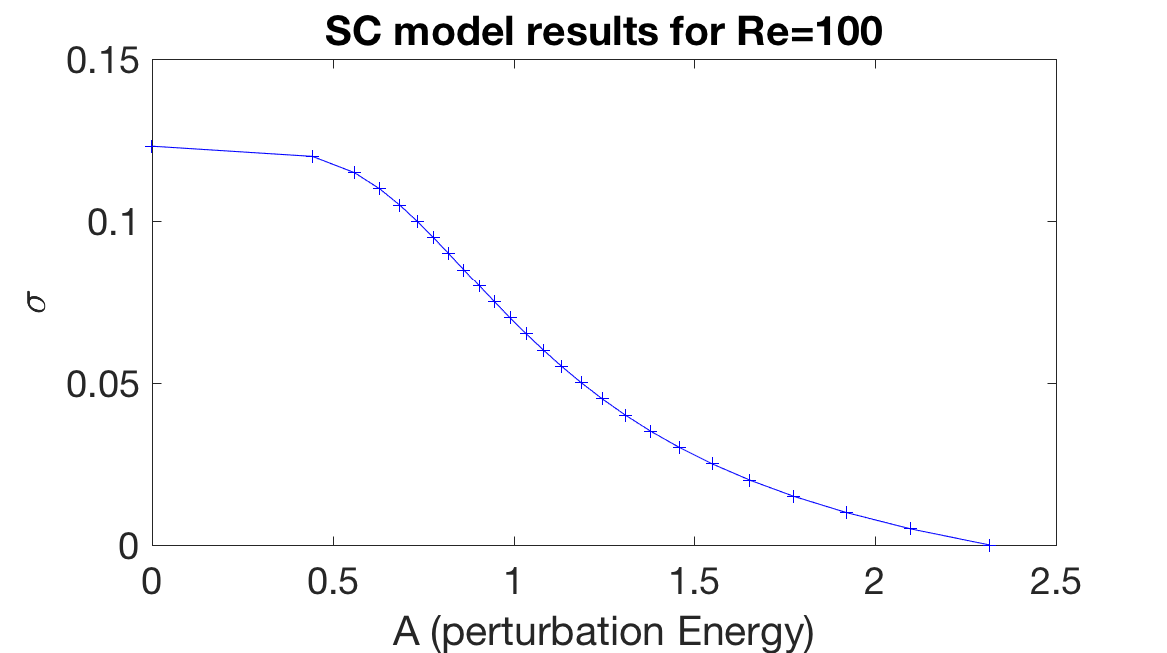
\includegraphics[width=\linewidth]{Cylinder_SC100_EnergySigma.png}
%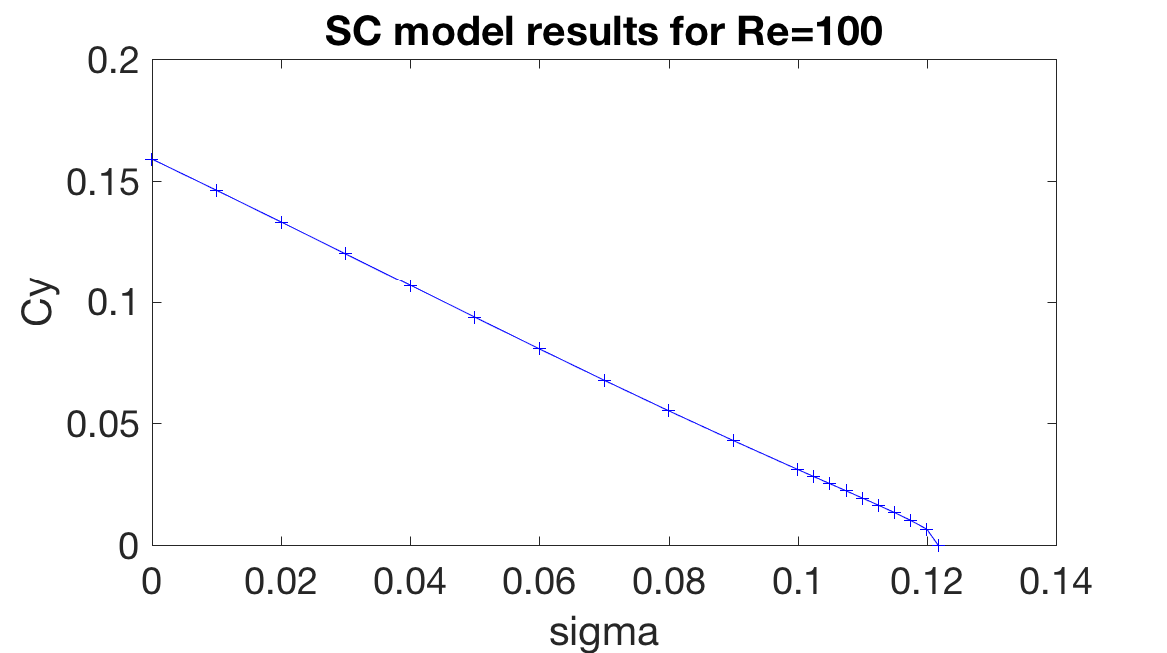
\includegraphics[width=\linewidth]{Cylinder_SC100_CySigma.png}
%\end{center}
%\caption{Self-consistent approach for the wake of a cyrcular cilinder: results at $Re =  100$.}
%\label{fig:SC100}
%\end{figure}


We now briefly review the self-consistent model as introduced by Manti\v{c}-Lugo et 
al. \cite{MLugo2014}.
In their original exposition, the authors adopted a pseudo-eigenmode expansion of the flow 
as follows: 
\be{SC}
{\bf u } = {\bf u }_m + A_{sc} \left[ \tilde{{\bf u }}_1 e^{\sigma_{sc} t + i \omega_{sc} t} +   \overline{\tilde{\bf u }_1} e^{\sigma_{sc} t  -i \omega_{sc} t} \right],
\ee  
where ${\bf u }_m$ is the {\em mean flow} as previously defined, $\tilde{{\bf u }}_1$ is a pseudo-eigenvector which is normalized by the condition  $||\tilde{{\bf u }}_1|| = 1/\sqrt{2}$, $\overline{\tilde{{\bf u }}_1}$ is its complex conjugate,
$A_{sc}$ is an amplitude parameter directly related to the energy of the oscillating flow, and $\lambda_{sc} = \sigma_{sc} + i \omega_{sc}$ is a pseudo-eigenvalue which depends upon the parameter $A_{sc}$. 

The original version of the model (discussed in detail in appendix C) allowed to obtain an amplitude equation predicting the instantaneous growth rate $\sigma$ as function of the amplitude $A_{sc}$. However, if we are simply interested in the properties of the limit cycle, not the transient, we may recast the self-consistent model in a simpler way.



We thus start with a truncated Fourier decomposition of the limit cycle under the form:
\be{HB}
{\bf u } = {\bf u }_m + {\bf u }_{1,c} \cos( \omega t ) +   {\bf u }_{1,s} \sin( \omega t ),
\ee
where ${\bf u }_{1,c}$ and ${\bf u }_{1,s}$ are two {\em real} fields describing the nonlinear perturbation at two instants separated by a quarter-period of oscillation, and $\omega$ is the (real) oscillation frequency of the limit cycle (which is not known a priori).  

Injecting this ansatz into the Navier--Stokes equations and taking the mean value and the first Fourier component leads to the following coupled equations:
\begin{subequations}\label{eq_principal}
\begin{eqnarray}
{\cal NS}(  {\bf u }_m ) = \frac{{\cal C}( {\bf u }_{1,c}, {\bf u }_{1,c}) +{\cal C}( {\bf u }_{1,s}, {\bf u }_{1,s})}{4}, 
\label{HBEq0}
\\
 \omega {\bf u }_{1,s} =  {\cal LNS}_{{\bf u }_m}(  {\bf u }_{1,c} ),
\label{HBEq1}
\\
 -\omega {\bf u }_{1,c} =  {\cal LNS}_{{\bf u }_m}(  {\bf u }_{1,s} ).
\label{HBEq1b}
\end{eqnarray}
\end{subequations}

%Note {\color{red} that,} contrary to the SC model, the amplitude $A_{HB}$ of the oscillation} can easily be computed a posteriori as ${\color{red}A_{HB}} = \sqrt{2 ||{\bf u }_1||}$. 
%On the other hand, the Fourier description of the limit cycle is invariant with respect to the phase $\phi$ (\textit{i.e.} the equations are unchanged when replacing ${\color{red} {\bf u }_1 }$ by  ${\color{red} {\bf u }_1 e^{i\phi}}$). 

Note that this system of equations contains three unknown fields (discretized on the Taylor--Hood basis) plus an extra scalar unknown, 
namely the frequency $\omega$. 
In order to solve this coupled problem, we thus need an extra scalar equation. The latter is provided by fixing the {\em phase} of the cycle. Several choices are possible, but a convenient one is to decide that the instant $t=0$ corresponds to a maximum of the lift force.
This condition reads:
\be{HBphase}
{\cal L}_{Re}({\bf u}_{1s},p_{1s}) =0, 
\ee
so that the Fourier decomposition of the lift force \eqref{drag_lift_def} will contain only a cosine term, namely 
\be{FySC}
F_y \approx F_{y,1,c} \cos \omega t, \quad \mbox{ with } \quad F_{y,1,c} = {\cal L}_{Re}({\bf u}_{1c},p_{1c}).
\ee 


Note that the amplitude $A_{sc}$, which was considered as a key parameter in the original model of \cite{MLugo2014}, 
does not appear in the simplified version discussed here. The connection between our parametrization and that of Manti\v{c}-Lugo et al. is as follows:
\be{HBtoSC}
\left( {\bf u }_{1,c} - i {\bf u }_{1,s} \right) = 2 A_{sc} \tilde{{\bf u }}_1.
\ee 
Considering their normalization choice, the parameter $A_{sc}$ of \cite{MLugo2014} can be easily deduced from our results as follows:
$A_{sc} = \sqrt{2 \int_\Omega ( |{\bf u }_{1,c}|^2+ |{\bf u }_{1,s}|^2) d S} $.








\paragraph{SC/HB1 model: a direct algorithm }


When reformulated in this way, the nonlinear problem addressed by the self-consistent model actually reduces to the restriction to order one of a more general class of methods called harmonic balance methods (HB).
One of the first applications of these methods in the domain of fluid mechanics has been done by Carte and Du\v{s}ek \cite{CarteDusek1995,CarteDusekfraunie1996}.
The development of such methods, or related ones such as the time-spectral method (\cite{HallThomasClark2002}) and the search for efficient numerical implementation to solve such problems is currently an active field of development in the fluid dynamics community.
When considering HB development with a large order of terms, direct resolution by inversion of the full matrix is not achievable. Methods including iterative solvers and efficient preconditioning are currently under development (O. Marquet, personal communication).

On the other hand, when restricting as here to a truncation to order one (HB1 method), the use of adapted meshes makes the building and inversion of the matrix accessible on standard computers.
We thus propose here a simple algorithm based on a direct resolution using a Newton iteration, just as explained for the base flow in section 2. This method is proposed as an efficient alternative compared to the double-loop resolution procedure of \cite{MLugo2014}.

The algorithm assumes that we know a {\em guess} for the full state-vector defined as follows:
$$
[{\bf u }_m, {\bf u }_{1,c}, {\bf u }_{1,s}, \omega] = 
 [{\bf u }_m^g, {\bf u }_{1,c}^g, {\bf u }_{1,s}^g, \omega^g]
+ [\delta {\bf u }_m, \delta {\bf u }_{1,c}, \delta {\bf u }_{1,s}, \delta \omega].
$$
Injecting and developing up to linear order leads to the following equations:
\iffalse
\begin{subequations}\label{eq:harmonic_total}
\begin{eqnarray}
\begin{split}
&{\cal NS}(  {\bf u }_m^g ) - \frac{1}{4} \big[ {\cal C}( {\bf u }_{1,c}^g,{\bf u }_{1,c}^g) +  {\cal C}( {\bf u }_{1,s}^g,{\bf u }_{1,s}^g) \big]+ {\cal LNS}_{{\bf u }_m^g}(\delta {\bf u }_m)
\\
&-\frac{1}{2} \big[ {\cal C}( {\bf u }_{1,c}^g,\delta {\bf u }_{1,c}) +  {\cal C}( {\bf u }_{1,s}^g,\delta {\bf u }_{1,s}) \big] = 0,
\end{split}
\label{HB_1}
\\
\begin{split}
{\cal LNS}_{{\bf u }_m^g}( {\bf u }_{1,c}^g) - \omega^g {\bf u }_{1,s}^g& -  {\cal C}( \delta {\bf u }_{m}, {\bf u }_{1,c}^g)
\\
&+{\cal LNS}_{{\bf u }_m^g}( \delta {\bf u }_{1,c})  - \omega^g \delta {\bf u }_{1,s}  
 - \delta \omega {\bf u }_{1,s}^g = 0 ,
 \end{split}
\label{HB_2}
\\
\begin{split}
{\cal LNS}_{{\bf u }_m^g}({\bf u }_{1,s}^g) + \omega^g {\bf u }_{1,c}^g& -  {\cal C}( \delta {\bf u }_{m}, {\bf u }_{1,s}^g)
\\
&+{\cal LNS}_{{\bf u }_m^g}( \delta {\bf u }_{1,s}) + \omega^g \delta {\bf u }_{1,c} +  \delta \omega {\bf u }_{1,c}^g= 0 ,
\end{split}
\label{HB_3}
\\
\begin{split}
 F_y({\bf u }_{1,s}^g) + F_y(\delta {\bf u }_{1,s}) = 0. \qquad \qquad \qquad \qquad \qquad \qquad \quad
\end{split}
\end{eqnarray}
\end{subequations}
\fi


\begin{subequations}

\begin{align}
{\cal NS}(  {\bf u }_m^g ) - \frac{1}{4} &\big[ {\cal C}( {\bf u }_{1,c}^g,{\bf u }_{1,c}^g) +  {\cal C}( {\bf u }_{1,s}^g,{\bf u }_{1,s}^g) \big]+ {\cal LNS}_{{\bf u }_m^g}(\delta {\bf u }_m) \nonumber \\
-\frac{1}{2}& \big[ {\cal C}( {\bf u }_{1,c}^g,\delta {\bf u }_{1,c}) +  {\cal C}( {\bf u }_{1,s}^g,\delta {\bf u }_{1,s}) \big] = 0, \label{HB_1} \\
{\cal LNS}_{{\bf u }_m^g}( {\bf u }_{1,c}^g)& - \omega^g {\bf u }_{1,s}^g -  {\cal C}( \delta {\bf u }_{m}, {\bf u }_{1,c}^g) \nonumber \\
&\hspace{-0.9cm}+{\cal LNS}_{{\bf u }_m^g}( \delta {\bf u }_{1,c})  - \omega^g \delta {\bf u }_{1,s}  
 - \delta \omega {\bf u }_{1,s}^g = 0 , \label{HB_2}\\
{\cal LNS}_{{\bf u }_m^g}({\bf u }_{1,s}^g)& + \omega^g {\bf u }_{1,c}^g -  {\cal C}( \delta {\bf u }_{m}, {\bf u }_{1,s}^g) \nonumber \\
&\hspace{-0.9cm}+{\cal LNS}_{{\bf u }_m^g}( \delta {\bf u }_{1,s}) + \omega^g \delta {\bf u }_{1,c} +  \delta \omega {\bf u }_{1,c}^g= 0 , \label{HB_3} \\
&\hspace{1.65cm} F_y({\bf u }_{1,s}^g) + F_y(\delta {\bf u }_{1,s}) = 0. 
\end{align}
\end{subequations}

After discretization, this leads to a linear problem of the form $A X = Y$ where $X$ is the discretized version of the unknowns  $[\delta {\bf u }_m, \delta {\bf u }_{1,c}, \delta {\bf u }_{1,s}, \delta \omega]$, and $A$ is a matrix of dimension $3 N_{dof} +1$, where $N_{dof}$ is the dimension of the Taylor--Hood basis of finite elements describing each of the three $[{\bf u},p]$ fields. This system is solved iteratively as explained in section 2.1 for the determination of the base flow. %Using the adapted mesh described in figure 2, the dimension of the system is $3 N_{dof} +1 \approx 58 000$ and the resolution remains possible at very reasonable computational costs. 
Mesh convergence issues for the nonlinear calculations are discussed in appendix A. It is shown that the mesh $\mathbf{M}_2$ designed using "S" strategy is sufficient to yield converged results within $0.3\%$ accuracy for all quantities considered here, with the exception of the energy-amplitude $A_E$ which requires the more refined mesh $\mathbf{M}_4$ obtained using "D" strategy.\footnote{In terms of computational cost, on a standard laptop the program  \ref{fig:listingNL} requires approximatively 7 minutes using  mesh $\mathbf{M}_2$ and 31 minutes using mesh $\mathbf{M}_4$.} 
 
In the proposed implementation, resolution of the problem is done by the FreeFem++ program {\sf  HB1\_2D.edp} which is wrapped by the Octave/Matlab function {\sf  SF\_HB1.m}.
Note that the interested reader will also find within the sources of StabFem project a driver {\sf  SF\_HB2.m} implementing the same direct resolution method for the order-2 truncated harmonic balance.
Generalization to higher orders is planned for future developments of the project.
  
 \paragraph{Results for the cylinder's wake}
 
Lines 10-17 of the script shown in figure \ref{fig:listingNL} explain how to use these programs to the SC/HB1 model for the wake of a cylinder in the range $Re \in [47-100] $. Note that a {\em guess} for the mean flow and the self-consistent mode for $Re = 47$, \textit{i.e.} just above the threshold, has already been generated from the weakly nonlinear model at line 4 of the same script. This guess is used for the first step of the loop over Reynolds in lines 14-17. For next steps of the loop, continuation is done using the previous calculation results as guess.

\begin{figure}
\begin{center}
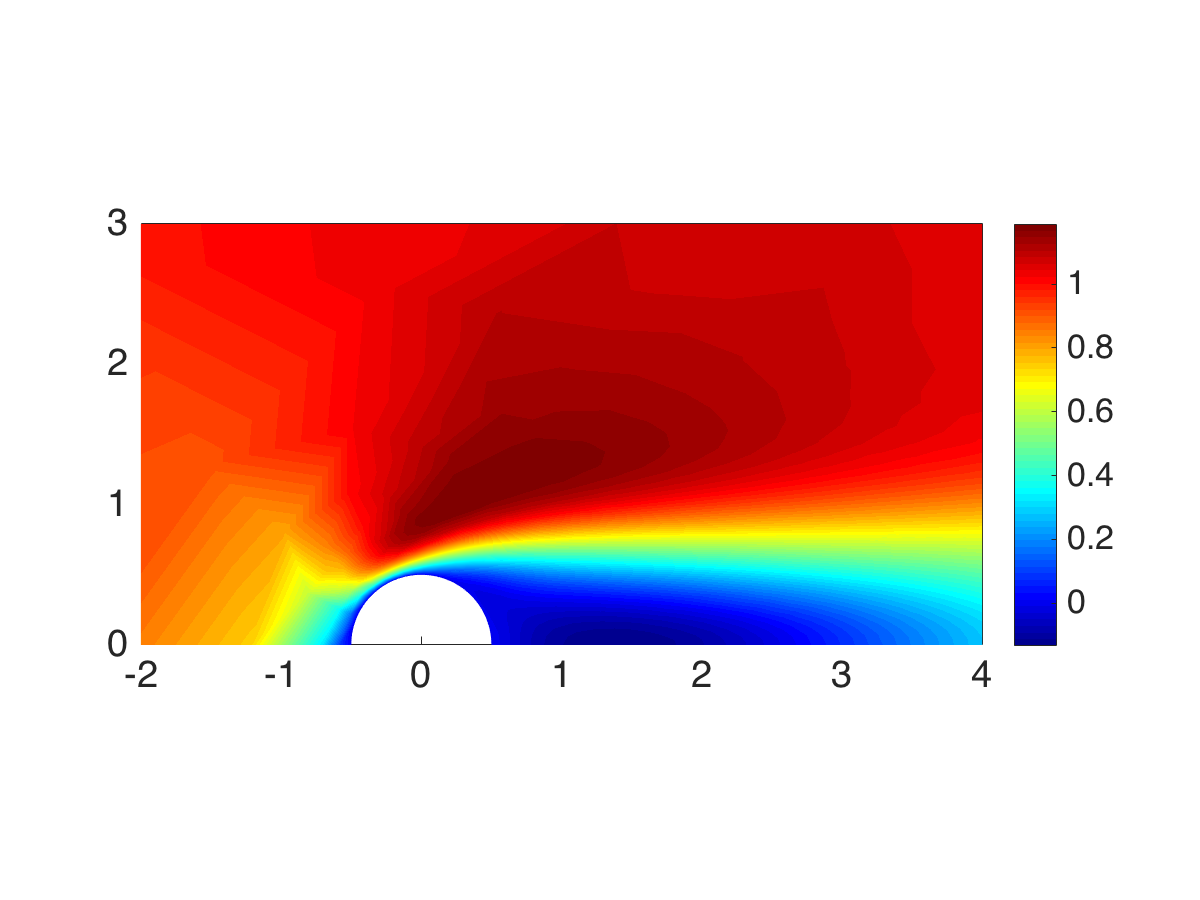
\includegraphics[width=\linewidth]{Cylinder_MeanFlowRe60.png}
\end{center}
\caption{Structure of the {\em mean flow} over a cylinder for $Re = 60$, as computed by the HB1 model. color levels: pressure ; streamlines.}
\label{fig:MF60}
\end{figure}



Figure \ref{fig:MF60} illustrates the structure of the mean flow for $Re=60$.
As already identified by  \cite{MLugo2014}, the recirculation region associated with this mean flow is notably shorter than the one associated with the base flow (figure \ref{fig:Baseflow}). 


%Line 19 shows how to plot the results along with the 
%\ref{HBEq0,HBEq1,HBphase}

Figure \ref{fig:HB_SC_DATA_COMP} shows the comparison between the WNL (green) and HB1/SC (red) models for the quantities of interest identified in this paper, namely the Strouhal number, the mean drag, the maximum lift, the energy-amplitude, and the recirculation length associated to the mean flow. When relevant, results regarding the base flow and the linear approach are also displayed (blue)
\footnote{Figure   \ref{fig:HB_SC_DATA_COMP} is obtained by line 19 of the script displayed in figure \ref{fig:listingNL}. The other figures are processed in a similar way. The entire set of commands to obtain all figures is provided in the script {\sf SCRIPT\_CYLINDER\_ALLFIGURES.m}.}.
Concerning the quantities $St$, $A_E$ and $L_x$, differences between HB1/SC, WNL models have already been commented in \cite{MLugo2014} and \cite{FDR2016}. 

%replace this paragraph by a description of figures displaying the comparison

The present results are also compared with the available literature, namely with the experiments of \cite{williamson1988defining} for the $St$ number and with the DNS results of \cite{MLugo2014} for $A_E$ and $L_x$.
The predictions of the SC/HB1 model show an excellent agreement in the range $Re \in [Re_c,100]$ with the references. %Regarding the forces exerted on the body, 
However, we can remark that the predictions of the WNL model rapidly depart from the previous ones as soon as $Re-Re_c \gtrsim 1$.

%Comparison of these results with DNS simulations is not provided here (consistently with the objectives of the present paper) but the reader may verify that the SC model correctly predicts these quantities in the range of Reynolds number considered here.



%\clearpage

\section{Conclusion}
%The aim of the present review is to introduce advanced stability approaches 
%from a {\tt practical} point of view. The reader can reproduce all the figures presented 
%in this paper by just running the Octave/Matlab code available in the StabFem repository. 


The objective of this paper is twofold. First, we aimed at giving an up-to-date and comprehensive review on global stability approaches, both linear and nonlinear, including the most recent developments of the field. 
Secondly, we intended to provide an easy to use software performing all these computations from a single program.
In accordance with this objective, all the figures presented in the paper can be produced by launching a single Octave/Matlab program available on the website of th project.
This program handles all computation steps, from calls to FreeFem++ to figure generation.

Although the focus here was on the reference case of 2D incompressible and compressible flow around a cylinder, the {\em StabFem } software is designed to be easily customisable to a variety of other situations.
The project is currently in constant development, and incorporates a growing number of other configurations.
Under its present status, the project incorporates test-cases for the following classes of problems:
\begin{itemize}
\item[-] Incompressible flows around 2D and axisymmetric blunt bodies of various geometries, including spheres and disks \cite{Tchoufag2015}. 
\item[-] Incompressible flows around 2D and 3D objects in free movement, including for instance the spring-mounted cylinder \cite{Navrose}, and freely falling disks and spheres \cite{tchoufag2014global}.
\item[-] Incompressible and compressible flow flow through apertures \cite{FabreISMA,longobardi2018IUTAM}, 
\item[-] Compressible flow around 3D objects  \cite{meliga2010effect},
\item[-] Oscillations of hanging drops, sessile drops and liquid bridges \cite{Chireux2015},
\item[-] Rotating free surface flows \cite{mougel2017instabilities}.
\end{itemize}
Our ambition is to use the website of the project as a support to publish scripts allowing anyone to reproduce the main results of our past and future publications
on such topics.  Such scripts are already available concerning Refs. \cite{Tchoufag2015,longobardi2018IUTAM,Chireux2015,mougel2017instabilities} and the list of available case will be growing in the coming months.The project is intended as collaborative, so anyone who wants to contribute is welcome !





%\section*{Acknowledgements}

%J. Tchoufag, J. Mougel, O. Marquet, D. Sipp, 


\appendix


%The problem can be set into weak form by multiplying by multiplying Eq. \ref{Newton2} by a test function ${\bf v}$ and the associated divergence constraint by a test function $q$. After a few integration by parts we are led to:

%SECTION TO BE COMPLETED.

%We have to explain the integration by parts of the viscous term.




%\begin{eqnarray}
%\label{NewtonWeak}
%&\forall ({\bf v};q), \\
%\displaystyle &\int \left[ {\bf v} \cdot {\cal C}( {\bf u}_b^g , \delta {\bf u}_b) +  \nabla  \cdot \delta {\bf u}_b q -\nabla  \cdot {\bf v} \delta p_b
%+ \frac{2}{Re} {\bf D}(\delta {\bf u}_b): {\bf D}({\bf v}) \right]
%\nonumber
%\\
%\nonumber
%\displaystyle & + \int \left[ {\bf v} \cdot ( {\bf u}_b^g \cdot \nabla {\bf u}_b^g) 
%+ \nabla \cdot {\bf u}_b^g  q 
%- \nabla \cdot {\bf v} p_b^g
%+ \frac{2}{Re} {\bf D}({\bf u}_b^g): {\bf D}({\bf v}) \right] = 0 
%\end{eqnarray}


\section{Mesh convergence: efficiency of mesh adaptation and effect of domain size}
\begin{figure}
%\vspace{-.5cm}\vspace{-.5cm}
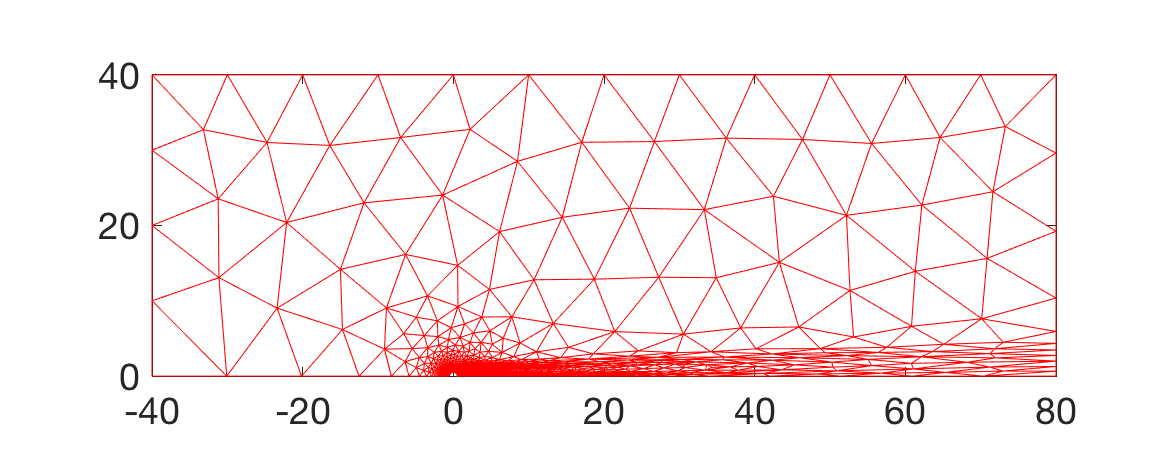
\includegraphics[width = .9\linewidth]{Cylinder_Mesh2_Full.png}
%\vspace{-.5cm}\vspace{-.5cm}
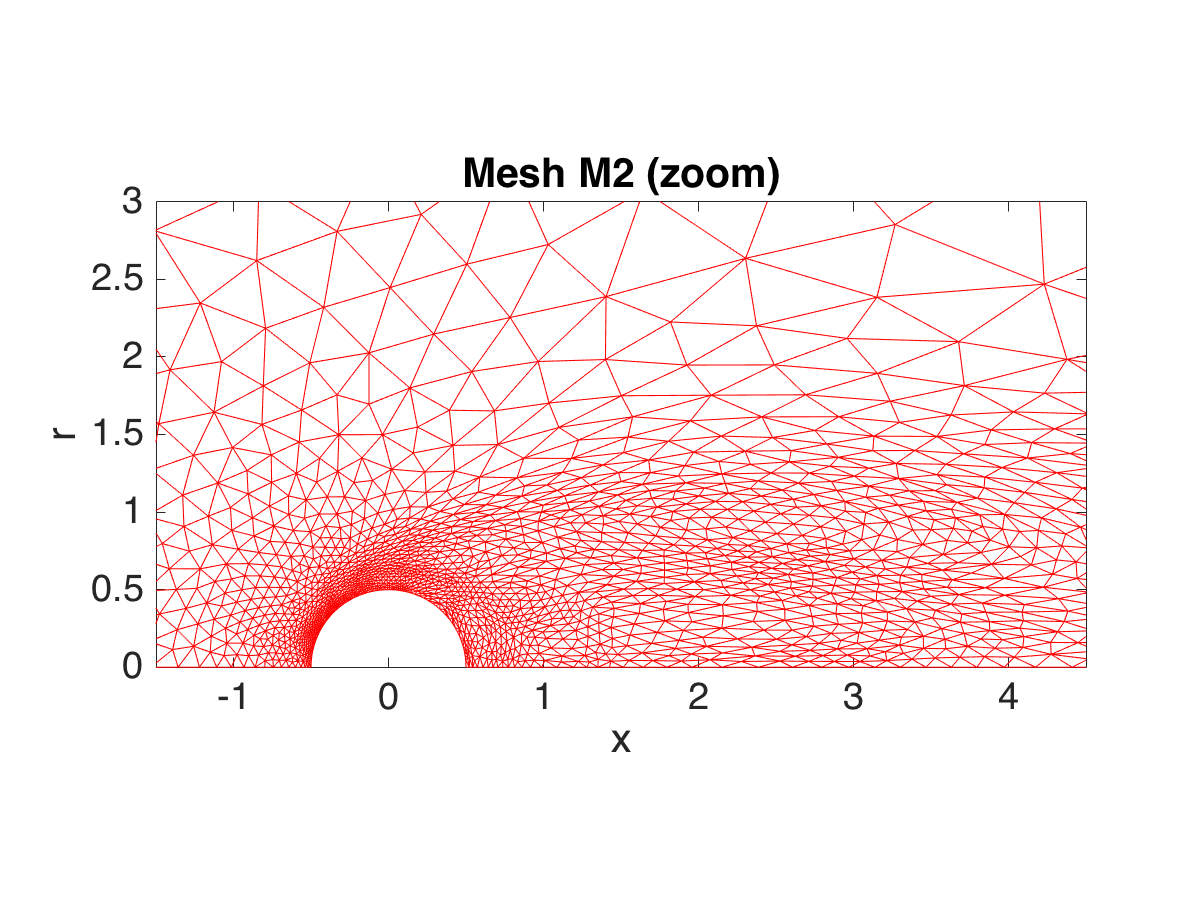
\includegraphics[width = .9\linewidth]{Cylinder_Mesh2.png}
\caption{Illustration of the stucture of mesh  $\mathbf{M}_2$ (adapted to both the base flow and structural sensitivity).}
\label{fig:mesh2}
\end{figure}

\begin{figure}
%\vspace{-.5cm}\vspace{-.5cm}
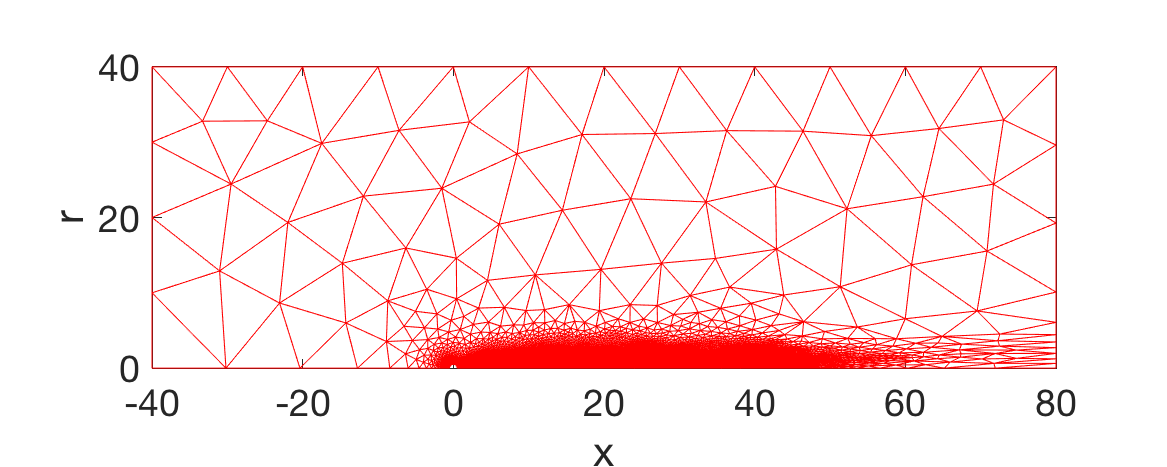
\includegraphics[width = .9\linewidth]{Cylinder_Mesh4_Full.png}
%\vspace{-.5cm}\vspace{-.5cm}
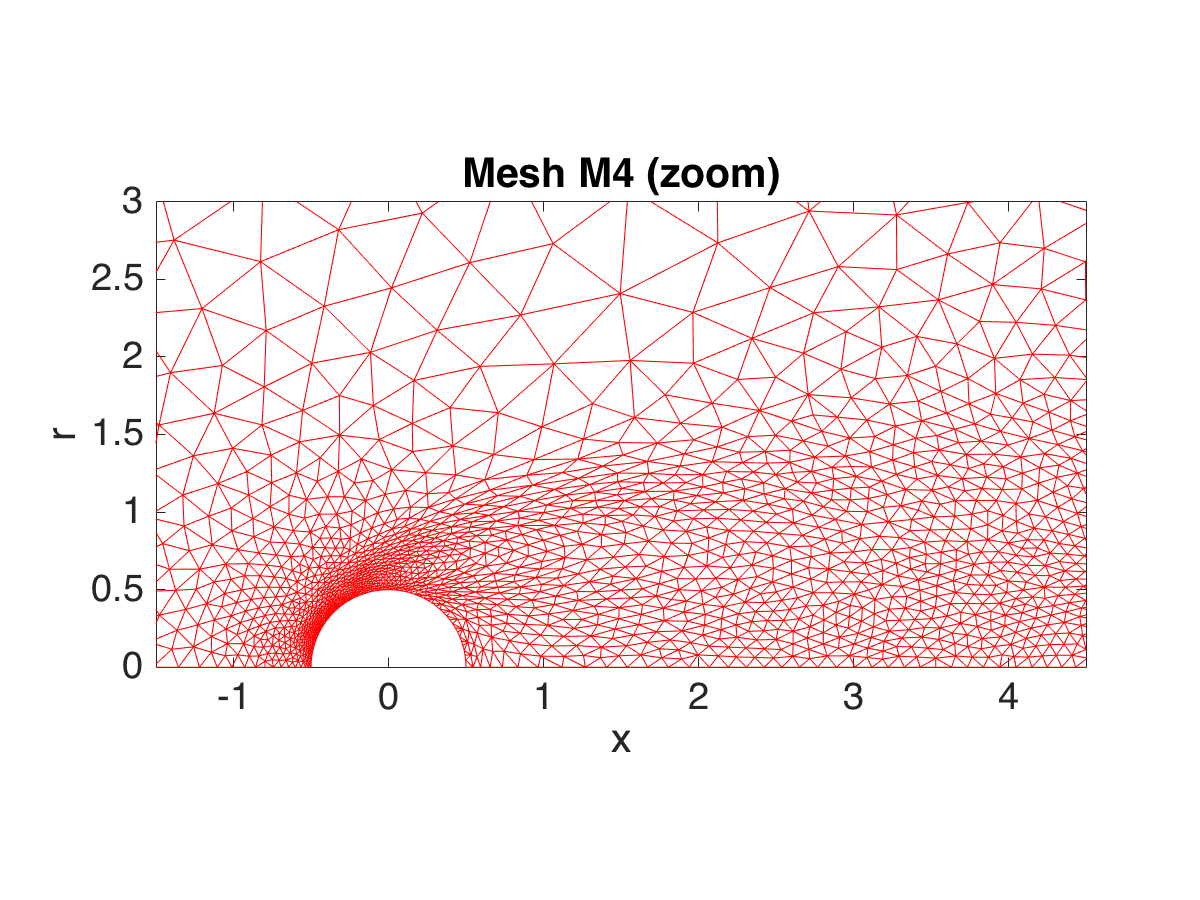
\includegraphics[width = .9\linewidth]{Cylinder_Mesh4.png}
\caption{Illustration of the stucture of mesh  $\mathbf{M}_4$ (adapted to both the base flow and direct eigenmode).}
\label{fig:mesh4}
\end{figure}



\begin{table*}
$$
\begin{array}{|c||c|c|c|c|c|c|c|c|c|}
\hline
\mbox{Mesh} & N_p & N_{dof} & \delta_{min} & \delta_{max} & \delta_A  & \delta_B  & \delta_C  & \delta_D  \\
\hline
\mathbf{M}_1 \mbox{(Adapt on base flow) } & 1429 & 12545	& 0.0131 & 14.33 		& 0.0259 	& 0.514 	& 0.819 	& 1.067 \\   
\mathbf{M}_2 \mbox{(Adapt on sensitivity) } & 2038 & 17885	& 0.0155 & 14.17 		& 0.02826 & 0.2046 	& 0.3909 	& 1.2014 	\\
\mathbf{M}_2' \mbox{(Adapt on sensitivity, split) } & 7974 & 70651	& 0.00786 & 7.131  		& 0.0104 	& 0.0744 	&   0.0975 & 0.614   \\
\mathbf{M}_3 \mbox{(Adapt following \cite{mavripilis2015adjoint}) } & 3749 & 32655	& 0.01542 & 12.7109  		& 0.09689 	& 0.1236 	&   0.2004 & 0.65775   \\
\mathbf{M}_4 \mbox{(Adapt on mode) } 	& 12080  & 103564		&0.00825	& 12.461		& 0.0229	& 0.143	& 0.0993	& 0.0934 \\
\mathbf{M}_5 \mbox{(Adapt on adjoint) } 	& 3813 	& 330715		& 0.0108	& 13.95		& 0.0176 	& 0.114	& 0.127	& 1.177  \\
\hline
\end{array}
$$
\caption{Description of meshes used for validation of mesh adaptation strategy: number of vertices $N_p$ ; number of degrees of freedom of the P2-P2-P1 Taylor--Hood basis $N_{dof}$ ; cell size (minimum and maximum value, and value at four characteristic point A,B,C,D as defined in the text). 
 }
\label{tab:conv1}
\end{table*}


%Fx = 0.6447; Lx = 4.0736
\begin{table*}
$$
\begin{array}{|c||c|c||c||c|c||c|c|c|}
\hline
\mbox{Mesh} & L_x & F_x & \lambda & L_{x,HB1} & F_{x,HB1} & \omega_{HB1}  & F_{y,1,c} & A_{E} \\
\hline
\mathbf{M}_1 & 4.0733 & 0.64310	& 0.047056 + 0.74416i 		& 2.6073  & 0.69277 	&  0.84334 & 0.1298 & 1.8301  \\
\mathbf{M}_2 & 4.075 &.  0.64348  	& 0.046719 + 0.74489i 		& 2.6153  & 0.69246 	& 0.84351 & 0.12789 & 1.7134 \\ 
\mathbf{M}_2' & 4.0772 & 0.64391 	& 0.04684 +  0.74511i 		& 2.6141  & 0.69338 	& 0.84383 & 0.12799 & 2.048   \\  
\mathbf{M}_3 & 4.0749 & 0.64370 	& 0.04673 + 0.74538i		& 2.6140     & 0.69317	& 0.84408 & 0.12808 & 2.064   \\ 
\mathbf{M}_4 & 4.0748 & 0.64402 	& 0.04676  + 0.74502i 		& 2.6130 	& 0.69034 	& 0.84371 & 0.12809 & 2.5905 \\
\mathbf{M}_5 & 4.0736 & 0.64470	& 0.046782+0.74534i		& 2.6142 	& 0.69399		& 0.84390 & 0.12800 & 1.8234 \\
\hline
\end{array}
$$
\caption{Results for mesh adaptation strategy ($Re = 60$): Base-flow characteristics $L_x$ and $F_x$, linear eigenvalue $\lambda$, 
Nonlinear self-consistent model characteristics  $\omega_{HB1}$, $F_{y,1,c}$ and $A_E$. All the results can be optained using the Octave/Matlab script
{\sf SCRIPT\_CYLINDER\_MESHCONVERGENCE.m}. }
\label{tab:conv2}
\end{table*}



This appendix presents complementary results obtained using various mesh designs. 
All results can be obtained using the following program available on the StabFem website: 
{\sf SCRIPT\_CYLINDER\_MESHCONVERGENCE.m}.

\subsection{Efficiency of the mesh adaptation process}

As discussed in section 3, the mesh adaptation proves to be an extremely efficient way to obtain significant and reliable results 
with very reasonable meshes.
The objective of this paragraph is to demonstrate this point by comparing the efficiency of several mesh adaptation ways. 

For this purpose, 6 meshes were generated. 
Mesh $\mathbf{M}_1$ was adapted on the {\em base flow} obtained for $Re=60$.
Mesh $\mathbf{M}_2$ was adapted to both the base flow and structural sensitivity (strategy S).
Mesh $\mathbf{M}_2'$ was obtained by a subsequent refinement of mesh $\mathbf{M}_2$, splitting all triangles in four subtriangles, therefore doubling the effective density of the mesh.
Mesh $\mathbf{M}_3$ was adapted to both the base flow and following \cite{mavripilis2015adjoint} (strategy E).
Meshes $\mathbf{M}_4$ and $\mathbf{M}_5$ were obtained by adapting to the structure of the direct eigenmode (strategy D) and of the adjoint eigenmode (strategy A). In each case, the adapt-mesh process was repeated twice to ensure a correct convergence.

Figures \ref{fig:mesh2} and \ref{fig:mesh4} illustrate the structure of meshes $\mathbf{M}_2$ and $\mathbf{M}_4$.
It can be observed that these two mesh-adaptation strategies lead to meshes with comparable densities in the region close to the cylinder.
On the other hand, when moving downwards in the wake, mesh $\mathbf{M}_2$ quickly gets rather coarse while mesh $\mathbf{M}_4$ maintains a significant density.

Table \ref{tab:conv1} gives numerical informations about the geometry of these meshes. In particular, we document the minimum and maximum cell size, as well as the cell size at four points A,B,C,D defined with by their coordinates as follows: $(x_A,y_A) = (0,0.5)$ (within the boundary layer at the cylinder wall); $(x_B,y_B) = (2.5,0.5)$ (in the region of maximum structural sensitivity); $(x_C,y_C) = (4,0)$ (in the near wake); $(x_D,y_D) = (10,0)$ (in the far wake).
Results confirm that all meshes have similar densities in the near wake (cell size at points A,B,C are comparable) while $\mathbf{M}_4$ has maximum resolution in the far wake (in the vicinity of point D).

Table \ref{tab:conv2} compares the results obtained with the six meshes.
For base-flow characteristics $L_x$ and $F_x$, all values agree with a relative dispersion of less than $0.15\%$.
This underlines that all adaptation strategies are successful to correctly compute the base flow. 
The performances of meshes for linear stability calculations can then be evaluated by comparing the eigenvalues.
Meshes $\mathbf{M}_2$ to $\mathbf{M}_5$ all give values within less than $0.1\%$ dispersion.
The value obtained with mesh $\mathbf{M}_1$, which is not adapted to the eigenmode, is a bit farther from the others but still rather good. The table also displays results allowing to compare the performances of meshes for nonlinear self-consistent calculations.
As for the frequency and the maximum lift, meshes $\mathbf{M}_2$ to $\mathbf{M}_5$ again give almost identical values within less than $0.1\%$ dispersion.
The dispersion concerning the energy-amplitude of the perturbation $A_E$ displayed in the last column is however much larger.
Only the mesh $\mathbf{M}_4$ is able to correctly compute this quantity, while all other meshes significantly underestimate it.
 This is not surprising since this quantity is an integral property which depends upon the structure of the nonlinear perturbation over the whole wake, not only the near-wake region.

From this study we can conclude that if we are only interested in predicting the frequency of the mode and the forces exerted on the cylinder (in both linear and nonlinear regimes), the strategies S (mesh $\mathbf{M}_2$) and E (mesh $\mathbf{M}_3$) are the most efficient and lead to a very light mesh (here only 2038 vertices for mesh $\mathbf{M}_2$). On the other hand, if we are interested in describing the structure of the perturbation in the whole domain (and being able to correctly evaluate its energy), mesh adaptation to the eigenmode structure is preferable.
However this second strategy produces a much finer mesh (here 12080 point).
 
 
 \begin{table*}
$$
\begin{array}{|c|c||c|c||c||c|c||c|c|}
\hline
\mbox{Mesh} & N & L_x & F_x & \lambda & L_{x,SC} & F_{x,SC} & \omega_{SC}  & F_{Y,SC} \\%& A_{E,SC} \\
\hline
%\mathbf{M}_2 \mbox{(ref)} 	& 7974  	& 4.0772 & 0.64391 	& 0.04684. +  0.74511i 	& 2.6141  & 0.69338 	& 0.84383 & 0.12799 & 2.048   \\ 
\mathbf{M}_6 [-20,40]x[0,20] 			& 1954	&  4.1097 & 0.65048 	& 0.048335+0.74989i 	& 2.6014  & 0.69988 & 0.85032 & 0.13219 \\%& 1.7019   \\ 
\mathbf{M}_7 [-80,160]x[0,80] 			& 2292	& 4.0618 & 0.64046		& 0.046081+0.74286i 	& 2.6188 	& 0.68924 	& 0.84042 & 0.12631 \\%& 1.6892 \\
\mathbf{M}_8 \mbox{("slip" conditions)}	 & 2026	& 4.0701 &0.64590		& 0.047017+0.74790i	& 2.6127 	& 0.69492		& 0.84613 & 0.12836 \\%& 1.7154 \\
\mathbf{M}_9 \mbox{("inlet" conditions)}	 & 2043	& 4.0677 &0.64	557	& 0.047077+0.74781i	& 2.6152 	& 0.69429		& 0.84562  & 0.12771 \\%1.7004 \\
\hline
\end{array}
$$
\caption{Comparison of the performances of several meshes with variable dimensions and different boundary conditions}
\label{tab:conv3}
\end{table*}






\subsection{Effect of domain size and boundary conditions}

As already identified in several previous studies, the size of the domain and the type of boundary conditions applied at the boundaries have a notable impact on results.
To illustrate this, we designed four additional meshes.
All were obtained through adaptation to base flow and sensitivity, just as mesh $\mathbf{M}_2$.
Meshes $\mathbf{M}_6$ and $\mathbf{M}_7$ are respectively twice smaller and twice larger than the reference one. 
Meshes $\mathbf{M}_8$ and $\mathbf{M}_9$ have the same dimension but the boundary condition at the lateral boundary $\Gamma_{lat}$ differs. 
Unlike the reference case $\mathbf{M}_2$ which uses a no-stress boundary condition (identical to that applied at the outlet), mesh $\mathbf{M}_8$ uses a "slip" condition $u_y = 0 ; \partial u_x/\partial y = 0$ while mesh $\mathbf{M}_9$ uses an even more restrictive constant-flow condition (the condition at the lateral boundary is $u_x = 1, u_y = 0$, just as for the inlet).
 
Even though the domain size of the reference case (namely $[-40,80]\times[0,40]$) may appear large, the table shows that confinement effects are still present. The quantity which appears to be the the most sensitive to domain size and/or boundary conditions is the imaginary part of the linear eigenvalue.
Interestingly, the nonlinear SC results appears to be more robust with respect to confinement effects than linear ones. 
In effect, values for nonlinear frequency $\omega_{SC}$ and the maximum lift $F_{y,1,c}$ obtained with meshes  $\mathbf{M}_2$, $\mathbf{M}_7$ $\mathbf{M}_8$ and $\mathbf{M}_9$ agree with less than $0.3\%$ dispersion.





\section{Additional details of the weakly nonlinear approach}

\subsection{Derivation of the amplitude equation using multiple-scale approach}

The initial derivation of \cite{SippLebedev} makes use of a multiple scale method in order to obtain an amplitude equation.
The starting point can be taken as the following expansion of the velocity flow field:
\be{WNL2}
\begin{aligned}
&{\bf u} = {}  {\bf u}_{bc} + \epsilon \left[ A_{wnl}(\tau)  \hat{\bf u} e^{i \omega_c t} + c.c. \right]\\
&+ \epsilon^2 \left[ {\bf u}_\epsilon + |A_{wnl}(\tau) |^2  {\bf u}_{2,0} + \left(  A_{wnl}(\tau) ^2 {\bf u}_{2,2} e^{2 i \omega_c t} + c.c. \right) \right]\\
& + {\cal O}( \epsilon ^3),
\end{aligned}
\ee
Note that compared to the simplified version given in the main text by eq. \eqref{WNL1}, the amplitude $A_{wnl}$ depends upon a slow time scale 
$\tau = \epsilon^2 t$.

Substituting the expansion \eqref{WNL2} into the Navier--Stokes equations \eqref{NSprimitive} and grouping terms multiplied by the same power of $\epsilon$, a hierarchy of equations is obtained. The order $\epsilon^0$ gives directly the base flow at $Re_c$. The order $\epsilon^1$
corresponds to the linear neutral eigenmode as computed in the first part of this article.
The order $\epsilon^2$ contains three terms respectively computed as the solutions of the following linear problems:
\begin{eqnarray}
 {\cal LNS}_{{\bf u}_{bc}} ({\bf u}_\epsilon) - 2 \nabla \cdot {\mathsf D}({\bf u}_{bc}) &=&0,
\label{eq:LL1} \\
{\cal LNS}_{{\bf u}_{bc}} ({\bf u}_{2,0}) &=& {\cal C}(\hat{\bf u},\overline{\hat{\bf u}}), \label{eq:LL2} \\
{\cal LNS}_{{\bf u}_{bc}} ({\bf u}_{2,2}) - 2 i \omega_c {\bf u}_{2,2}  &=& \frac{1}{2} {\cal C}(\hat{\bf u},\hat{\bf u}). \label{eq:LL3}
 \end{eqnarray}

Finally, compatibility conditions, given by the Fredholm's alternative, are imposed at order $\epsilon^3$ to remove the secular terms, leading to an amplitude equation, known as Stuart-Landau equation:
\be{WNL3_2}
\frac{\partial A_{wnl}}{\partial \tau} = \Lambda A_{wnl} - (\nu_0+\nu_2)  |A_{wnl}|^2 A_{wnl},
\ee
where coefficients $\Lambda$, $\nu_0$ and $\nu_2$ are given by
\begin{eqnarray}
\Lambda &=& -\frac{ \left< {\hat{\bf u}}^\dag, 
\left( {\cal C}({\bf u}_\epsilon, \hat{\bf u}) + 2 \nabla \cdot  {\mathsf D}( \hat{\bf u}) \right) \right>}
{  \left<  \hat{\bf u}^\dag,\hat{\bf u} \right> },\label{LAMBDA}\\
\nu_0 &=& \frac{ \left< {\hat{\bf u}}^\dag,  {\cal C}({\bf u}_{20}, \hat{\bf u} ) \right>}
{  \left<  \hat{\bf u}^\dag,\hat{\bf u} \right> },\label{NU0}\\
\nu_2 &=& \frac{ \left< {\hat{\bf u}}^\dag,  {\cal C}({\bf u}_{22}, \overline{\hat{\bf u}})  \right>}
{  \left<  \hat{\bf u}^\dag,\hat{\bf u} \right> }.,\label{NU2}
 \end{eqnarray}


\subsection{Normalisation of the eigenmode}

\begin{table*}[!h]
\centering
$$
{\small
\begin{array}{|c||c|c|c|c|c|c|c|c|}
\hline
\mbox{Norm.} & \lambda & \nu_{0} & \nu_{2} &\omega_{\epsilon}& F_{x,0,\epsilon} & F_{y,1,c}/\epsilon & F_{y,1,s}/\epsilon &  |F_{y,1}| /\epsilon \\
\hline
\mbox{\cite{SippLebedev}} & 9.10988+3.28004i & 9.3996-32.0289i & -0.305116-0.866118i & 36.2307 
& 5.2848 & 0.0349973 & -0.536113 & 0.537254
\\
\mbox{\cite{FDR2016}} &  9.10988+3.28004i  & (0.488701 -1.66524 i) \times 10^{-3} & (-1.58635 - 4.50309i )\times 10^{-5} &36.2307
& 5.2848 & 0.537254 & 0 & 0.537254
\\
\mbox{\cite{Fabre2008}} & 9.10988+3.28004i & 32.62-111.152i & -1.05886-3.00574i & 36.2307
& 5.2848 & 0.537254 & 0 & 0.537254
\\
\hline
\end{array}
}
$$
\caption{Results of the WNL approach for three different choices of eigenmode normalization.}
\label{tab:WNL_coefs}
\end{table*}



A key issue in the weakly nonlinear expansion is that the definition of the amplitude depends upon a normalization choice of the eigenmodes. Several choices are possible.
In the literature three possibilities have been used:
%\begin{itemize}
%\item 

First, \cite{SippLebedev} normalized the eigenmode by assuming a specified value to the $y$-component of the velocity at one point, namely:
\be{normsipp}
\hat{u}_y(1,0) = 0.4612.
\ee
The advantage of this choice is that the coefficients $\nu_0$ and $\nu_2$ have the same order of magnitude as the coefficient $\Lambda$.

%\item 
Secondly, \cite{FDR2016} proposed the following normalization choice:
\be{normFDR}
\int_\Omega |\hat{\bf u}|^2 d {\bf x}  = \frac{1}{2}.
\ee
This directly leads to $|A| = A_E$, so this normalisation seems equivalent to the previous one.
%{\color{red} The lift phase is not specified in \cite{FDR2016} and can be set to nil before the normalization.}

%\item 
Thirdly, following \cite{Fabre2008}, another convenient choice is to normalize the eigenmode with its lift 
force: 
\be{normfabre}
{{\cal D}_{Re_c}(\hat{\bf u},\hat{p}) }=\frac{1}{2}.
\ee
The advantage of this choice is that the amplitude $|A|$ is then a direct measure of the fundamental lift.
In effect, eq. \eqref{lift_cos} directlty leads to $F_{y,1,c} = |A|$, $F_{y,1,s} = 0$. 


In our implementation of the WNL approach, we allowed choosing the normalization convention, as seen in line 4 of figure \ref{fig:listingNL}.
%%ATTENTION, si figure est actualisé, il faut actualiser la ligne
In table \ref{tab:WNL_coefs} we give the predictions of the WNL approach using the three normalization choices.
We can note that the coefficients $\nu_0$ and $\nu_2$ strongly depend on the normalization choice. On the other hand, the frequency deviation $\omega_\epsilon$, the $\lambda$ coefficient, and the term $F_{x,0,\epsilon}$ related to the dependency of mean drag with deviation from the threshold are independent upon the normalization.

Considering the lift force, columns 7 and 8 of the table show that the different choices of normalization give different values for the coefficients $F_{1,y,c}$ and $F_{1,y,s}$. %This explains that the normalization choice fixes differently the phase of the cycle. 
However,  the sin-cos expansion of the lift force can be recast as 
$F_y =  (F_{y,1,c} \cos \omega t + F_{y,1,s} \sin \omega t ) =  |F_{y,1}|  \cos (\omega t + \varphi)$ 
with $ |F_{y,1}| =  \sqrt{F_{y,1,c}^2 + F_{y,1,s}^2}$. The last column of the table confirms that the three possible normalization choices effectively lead to the same values of $|F_{y,1}|$.


%\be{lift_explanation}

%= {\color{red}|A|} \left( {\color{red}\frac{1}{2}} e^{i \omega t} + c.c. \right)
%=   {\color{red}|A|} \cos (\omega t) ; \quad F_{y,1,{\color{red}s}} = 0. 
%\ee

%\end{itemize}





\section{Additional details about the self-consistent method}

The objective of this appendix is to provide additional details about the SC model in its original form as given by \cite{MLugo2014}, and to explain the connection with the simpler version discussed in section 4.2.
The full model is obtained by introducing the decomposition \eqref{SC} into the Navier--Stokes equations, leading to:
\begin{subequations}\label{sc12}
\begin{eqnarray}
{\cal NS}(  {\bf u }_m ) - A^2 {\cal C}( \tilde{{\bf u }}_1, \overline{\tilde{\bf u }_1}) = 0, 
\label{sis1}
\\
(\sigma_{sc} + i \omega_{sc}) \tilde{{\bf u }}_1 =  {\cal LNS}_{{\bf u }_m}(\tilde{{\bf u }}_1 ).
\label{sis2}
\end{eqnarray}
\end{subequations}

Equation \eqref{sis1} provides the mean flow field ${\bf u }_m$ while the 
pseudo-eigenpairs $(\lambda_{sc},  \tilde{{\bf u }}_1)$ can be computed by solving the eigenvalue problem \eqref{sis2}.
\cite{MLugo2014} initially proposed a resolution method involving two nested loops, which is advantageously replaced by
the direct Newton resolution of section 4.3. 

%The computed mode is normalized as $ || \tilde{{\bf u }}|| = 1/{\sqrt{2}}$
%is of the same form as  (\ref{HBEq1}) except that $i \omega$ is 
%replaced by $\sigma_{SC} + i \omega_{SC}$. 
% The mean flow is then governed by the same equation
%\ref{HBEq0}) written above, while $\tilde{{\bf u }}_1$ is the solution of an eigenvalue problem with the same form as  (\ref{HBEq1}) except that $i \omega$ is replaced by $\sigma_{SC} + i \omega_{SC}$.

The self-consistent model has the following properties:
\begin{itemize}
\item[-] For $ A \ll 1$, it is equivalent to the linear eigenvalue problem \eqref{LEP}, and the generalized eigenvalue coincides with the one predicted by linear stability: $\sigma_{SC} + i \omega_{SC} = \sigma_{lin} + i \omega_{lin}$.
\item[-] For $\sigma_{SC}=0$ (corresponding to a specific choice of the amplitude $A=A_{sc}$), the expansion \eqref{SC} is equivalent to 
the Fourier expansion \eqref{HB} taken as the starting point in the present paper. 
\item[-] For $0<A<A_{sc}$, the resolution leads to a relation $\sigma_{SC}(A) ; \omega_{SC}(A)$
such that $0< \sigma_{SC}(A) < \sigma_{lin}$.
 Although in this case the expansion ({\ref{SC}}) cannot represent the flow for all $t$, Manti\v{c}-Lugo et al \cite{MLugo2014} argued that the relation between $\sigma_{SC}$ and $A$ can be used to build an amplitude equation which captures the transient approach to the limit cycle. 
\end{itemize}

\lstset{language=c++,%
   %basicstyle=\color{red},
   breaklines=true,%
   morekeywords={c++},
   keywordstyle=\color{blue},%
   morekeywords=[2]{1}, keywordstyle=[2]{\color{black}},
   identifierstyle=\color{black},%
   stringstyle=\color{mylilas},
   commentstyle=\color{mygreen},%
   showstringspaces=false,%without this there will be a symbol in the places where there is a space
   numbers=left,%
   frame=trBL,
   numberstyle={\tiny \color{black}},% size of the numbers
   numbersep=9pt, % this defines how far the numbers are from the text
   emph=[1]{for,end,break},emphstyle=[1]\color{red}, %some words to emphasise
   %emph=[2]{word1,word2}, emphstyle=[2]{style},   
   }



\begin{figure*}[t]
\small
\lstinputlisting[firstline=2, lastline=19]{Extract_From_Stab2D.edp}
 \normalsize
\caption{Illustration of the implementation of the Newton algorithm for base-flow computation (extract from FreeFem++ program {\sf  Newton2D.edp}).}
\label{Listing3}
\end{figure*}



Note that in our numerical implementation, the programs can actually be used to solve the SC model in the general case (with $\sigma\ne0$). 
This can be controlled by assigning a nonzero value to the optional parameter \verb|sigma| of the  {\sf SF\_SelfConsistent.m} Octave/Matlab function. The interested reader will find on the website of the {\sf  StabFem} project a program {\sf SCRIPT\_CYLINDER\_NONLINEAR.m} which computes $A$ as function of $\sigma$ for $Re=100$, yielding identical results as displayed in figure 3 of \cite{MLugo2014}.

\section{Details of the weak formulation}

In the presentation of the numerical methods in sections 2.1 and 2.2, and introduction of the {\em weak form}, we have omitted an important point, namely the issue of boundary conditions. In this appendix we explain more rigorously how the weak formulation is obtained. We consider here the full time-dependent nonlinear Navier--Stokes equations, but the treatment of the base-flow equations and the linearised equations is essentially the same.

Noting $\Gamma$ the boundary of the numerical domain, the latter can be decomposed in five parts: 
$\Gamma = \Gamma_{in} \cup \Gamma_{cyl} \cup \Gamma_{axis} \cup \Gamma_{out} \cup \Gamma_{lat}$. 
Noting $\sigma = 2 Re^{-1} {\bf D}({\bf u}) - p {\bf 1}$ the stress tensor, the relevant boundary conditions are as follows:
\begin{itemize}
\item On $\Gamma_{in}$ (inlet): ${\bf u} = {\bf e}_x$ (Dirichlet).
\item On $\Gamma_{cyl}$ (surface of the cylinder): ${\bf u} = {\bf 0}$ (Dirichlet).
\item On $\Gamma_{out}$ (outlet): $\sigma \cdot {\bf n} = {\bf 0}$ (Neumann). 
\item On $\Gamma_{lat}$ (lateral boundary):  $\sigma \cdot {\bf n} = {\bf 0}$ (Neumann). 
\item On $\Gamma_{axis}$ (symmetry plane): $u_y = 0$ and $\sigma_{xy} = 0$ (Mixed). 
\end{itemize}
We will introduce the following notation for integrals along any portion of the boundary $\Gamma_i$ of the product of two quantities $\phi_1, \phi_2$ (either scalar or vectorial):
%$\left< \phi_1, \phi_2 \right>_{\Gamma_i} $:
$$
\left< \phi_1, \phi_2 \right>_{\Gamma_i} = \int_{\Gamma_i}  \overline{\phi}_1 \cdot \phi_2   \mbox{ d} \ell,
$$
Instead of the simplified version \eqref{NSweak}, the more precise form of the weak formulation can be first written as follows:
\begin{eqnarray}
\label{NSweakFull}
\forall [{\bf v},q], &&\quad \partial_t \left< {\bf v}, {\bf u}\right> = \left< {\bf v} , {\cal NS} ({\bf u},p) \right> + \left< q, \nabla \cdot {\bf u}\right>\\
+ &&\frac{1}{\epsilon} \left(  \left< {\bf v}, \bf{u} \right>_{\Gamma_{cyl}} + \left< {\bf v}, ({\bf u}- {\bf e}_x ) \right>_{\Gamma_{in}} 
+ \left< v_y, u_y\right>_{\Gamma_{axis}} \right) \nonumber \\
+ && \left< {\bf v}, \sigma \cdot {\bf n} \right>_{\Gamma_{out} \cup  \Gamma_{lat} \cup \Gamma_{axis} }  \nonumber 
\end{eqnarray}
where $\epsilon=10^{-30}$ is a small parameter used to impose the Dirichlet boundary conditions by penalization.
An integration by parts of the pressure gradient and viscous stress terms of the Navier--Stokes equation eventually 
leads to the weak form effectively used in the programs {\sf Newton2D.edp} and {\sf Stab2D.edp}:
\begin{eqnarray}
\forall [{\bf v},q], &&\, \partial_t \left< {\bf v}, {\bf u}\right> = - \left< {\bf v} , {\cal C}({\bf u},{\bf u})/2 \right>
- 2 Re^{-1} \left< {\mathsf D}({\bf v}): {\mathsf D}({\bf u})  \right>  \nonumber \\
+ &&\left< \nabla \cdot {\bf v}, p \right> + \left< q, \nabla \cdot {\bf u} \right> \label{NSweakFullN} \\
+ &&\frac{1}{\epsilon} \left(  \left< {\bf v}, \bf{u} \right>_{\Gamma_{cyl}} + \left< {\bf v}, ({\bf u}- {\bf e}_x ) \right>_{\Gamma_{in}} 
+ \left< v_y, u_y\right>_{\Gamma_{axis}} \right) \nonumber 
\end{eqnarray}
Note that the Neumann boundary conditions do not appear anymore thanks to the integration by parts.


\begin{figure*}[t]
\small
\lstinputlisting[firstline = 24]{Extract_From_Stab2D.edp}
 \normalsize
\caption{Illustration of the implementation of the shift-invert algorithm for single eigenmode computation (extract from FreeFem++ program {\sf  Stab2D.edp}).}
\label{Listing4}
\end{figure*}


\section{Numerical implementation in FreeFem++}

In this appendix, we provide pieces of codes illustrating how the basic algorithms are implemented in the FreeFem++ solvers.
These explanations will be useful both for readers who wish to use directly FreeFem++ solvers without using the overlayer of Octave/Matlab drivers provided by the StabFem software, and also for the reader who wants to understand the logics of the implementation and to customize the software to implement their own cases.
The full version of the codes is available in the web repository of the StabFem project.
A full documentation of the software is also in progress \footnote{\url{https://gitlab.com/stabfem/StabFem/blob/master/99_Documentation/MANUAL/main.pdf}}.

Figure \ref{Listing3} details the implementation of the Newton algorithm for base-flow computation, as implemented in the FreeFem++ solver {\sf  Newton2D.edp} which is a generic solver usable for the whole class of 2D incompressible problems.
Note that the syntax makes use of macros {\sf  D, div, Conv}, resulting in a very similar to the weak formulation written in the previous appendix. The boundary conditions are also implemented using a macro {\sf  BoundaryconditionsBaseFlow}.
To allow an easy customization, this macro is not defined in the generic solver {\sf  Newton2D.edp} but is reported in a file {\sf  Macros\_StabFem.idp} regrouping case-dependant macros (essentially boundary conditions and post-processing options).

Figure \ref{Listing4} details the implementation of the shift-invert algorithm for eigenvalue computation, as implemented in the generic solver {\sf  Stab2D.edp} for 2D incompressible flows.
Here again, boundary conditions (which may differ from a case to an other within the generic class of 2D incompressible flows) are defined by a macro {\sf  BoundaryconditionsStability} which has to be defined in the  {\sf  Macros\_StabFem.idp} file.

We do not provide here the listing for the Newton resolution of the HB1 model, but the interested reader is encouraged to look at the program {\sf  HB1\_2D.edp} on the project site.

%In this appendix we compare the results obtained with 8 different meshes, to demonstrate the efficency of the mesh adaptation process. The whole results can be obtained using the script {\em SCRIPT\_CYLINDER\_MESHCONVERGENCE.m} available in the StabFem repository.

%Giannetti \& Luchini\cite{GiannettiLuchini} showed that the accuracy of the stability results for the flow past a circular cylinder is strictly related to the mesh characteristics  in the wavemaker region, \textit{i.e.} the region where the structural sensitivity reaches its maximum values. Following this idea, we chose as reference solution the field, computed on an adapted mesh obtained by using the structural sensitivity field.We set the interpolation  error equal to 0.01 and the size of the computational domain is $[-40,120]\times[0,40]$. The base flow is computed by using classical no-slip boundary conditions on the body surface, a uniform velocity profile at the inlet and no-stress boundary conditions at the outlet and lateral boundaries. The conditions for the stability computations are simply derived from the ones of the base flow.

%Figure \ref{fig:MeshConvergence} displays global stability results. We note that there is a very weak variation in the growth rate and we found an error up to 1\% on the  Strouhal number. Figure \ref{ill_bsflow} illustrate the procedure adopted to compute the 
%base flow and the adapted mesh. Figure \ref{stabmesh} reports the Octave/Matlab code 
%adopted to adapt the mesh by using the information provided by both the base flow and the sensitivity field. 



%Figure 1 gives a retranscription of the sequence of commands (from {\em SCRIPT\_CYLINDER\_ADAPTMESH\_BASEFLOW}) 
%and the output produced.

\bibliographystyle{asmems4}

\bibliography{ARTICLE_ASME}

\end{document}
